\resetfigpath{Chap5}

%%%{INTRODUCTION to this CHAPTER}%%%
In this chapter, the applications of the proposed driver behavior model are presented. In the first application, the relationship between certain driver behaviors and crashing cases are identified. Then, the proposed model is applied to predict the behaviors of drivers at an urban crossroad in real world where the performance is also evaluated. For the second application, considering that in the near future, it will be urgent for autonomous vehicles to handle the stnad-off situation where both participants are having the intention to yield (or to pass). To provide evidence that the proposed method is able to identify such situation and allows drivers (both computer and human ) to make reasonable reactions accordingly, a simulated autonomous vehicle is constructed to predict the behavior of human driver based on the proposed POY model. Finally, the driver parameters at various crossroads in real world are also identified using the proposed model. Despite only the average parameters are acquired, these values are important factors for autonomous vehicles to travel through different crossroads.   


%%%%%%%%%%%%%%%%%%%%%%%%%%%%%%%%%%%%%%%%%%%%%%%%%%%%%%%%%%%%%%%%%%%%%%%%
%%%%%%%%%%               SECTION SECTION SECTION               %%%%%%%%%
%%%%%%%%%%%%%%%%%%%%%%%%%%%%%%%%%%%%%%%%%%%%%%%%%%%%%%%%%%%%%%%%%%%%%%%%



\section{Crash Examinations in the Simulated Crossroad}
\label{sec:CrashSim}

During the experiments in the simulated crossroad in Gazebo, few cases failed to cross the intersection safe and sound. In these cases, the participants either did not notice the oncoming vehicle from the left (or right) or misjudged the arriving time of the other vehicle (i.e. its TTC) and led to the crashes. To examine the cause of the accidents, first the TFA distributions of both participants and the average distribution are shown and explained. Then, POYs are also shown together with the TTC difference for further explanation. 

There are considerable number of reasons that can lead to crashes which seemly happen in a random pattern. However, there do exist some regions and intersections where traffic accidents happen more frequently. Reasons behind the high accident number might be the light conditions, the design of the road layouts or even the driving pattern of drivers in the neighborhood. In this section, these regions are attempted to be identified using the concept of the proposed TFA distribution. Then, the likelihood of accidents happening could also be estimated.

%%%%%%%%------------------------------%%%%%%%%%
%%%%%%%%-----------SUBSECTION---------%%%%%%%%%
%%%%%%%%------------------------------%%%%%%%%%
\subsection{Crashing Likelihood Using TFA Distributions}
In Chapter \ref{chap:DriverModel}, the TFA distribution is defined as the probability density function of the driver taking actions (e.g. braking) under different TTC. The closer the current TTC to the mean TFA of the driver, more likely the driver will brake at this TTC. As a consequence, in the \textbf{normal} cases (where vehicles passed or yield without collisions), drivers brake at TTCs within the TFA distribution to avoid potential collisions and most of the TTCs that drivers brake at are those closer to the mean value of the TFA distribution (those with higher likelihood). What can be noted here is that, as long as the TTC while braking is within the bound of the TFA distribution, greater the TTC value while braking stands for the more conservative driving pattern despite the smaller likelihood, and smaller the TTC value while braking represent the more aggressive driving pattern. To clarify the idea, let us look at the TFA distributions of a normal case where no accident happened (as shown in Fig.~\ref{fig:normal015} and Fig.~\ref{fig:TFAs_normal015}).

\begin{figure}[htbp!]
\begin{center}
\makebox[0pt]{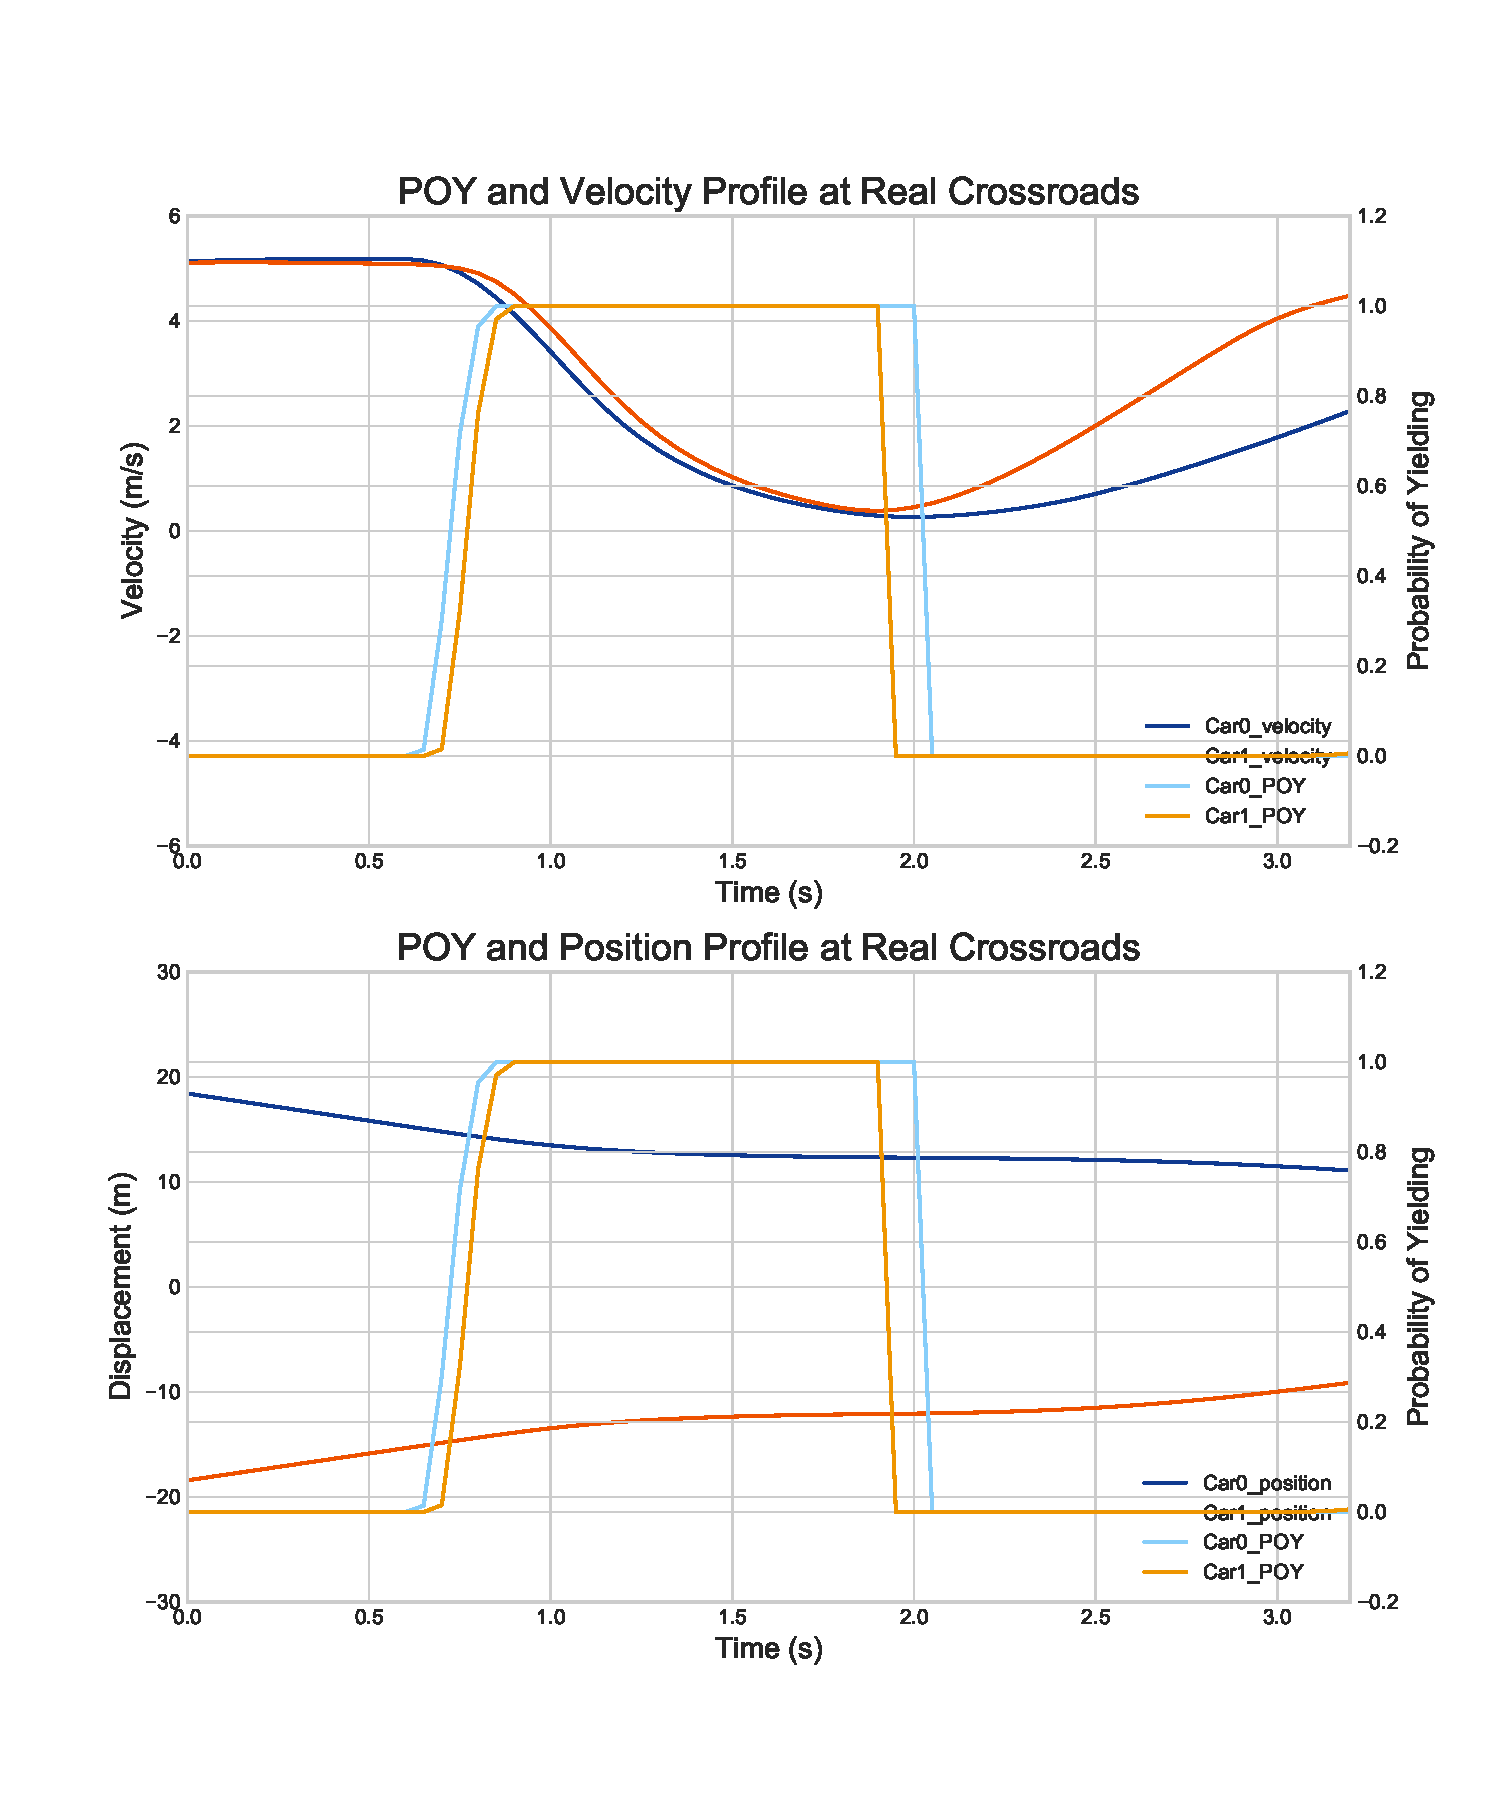
\includegraphics[width=0.65\paperwidth]{/normal_015.pdf}}
\end{center}
\caption{The velocities and displacements versus POYs of a normal case where no collision happened.}
\label{fig:normal015} 
\end{figure}

\begin{figure}[htbp!]
\begin{center}
\makebox[0pt]{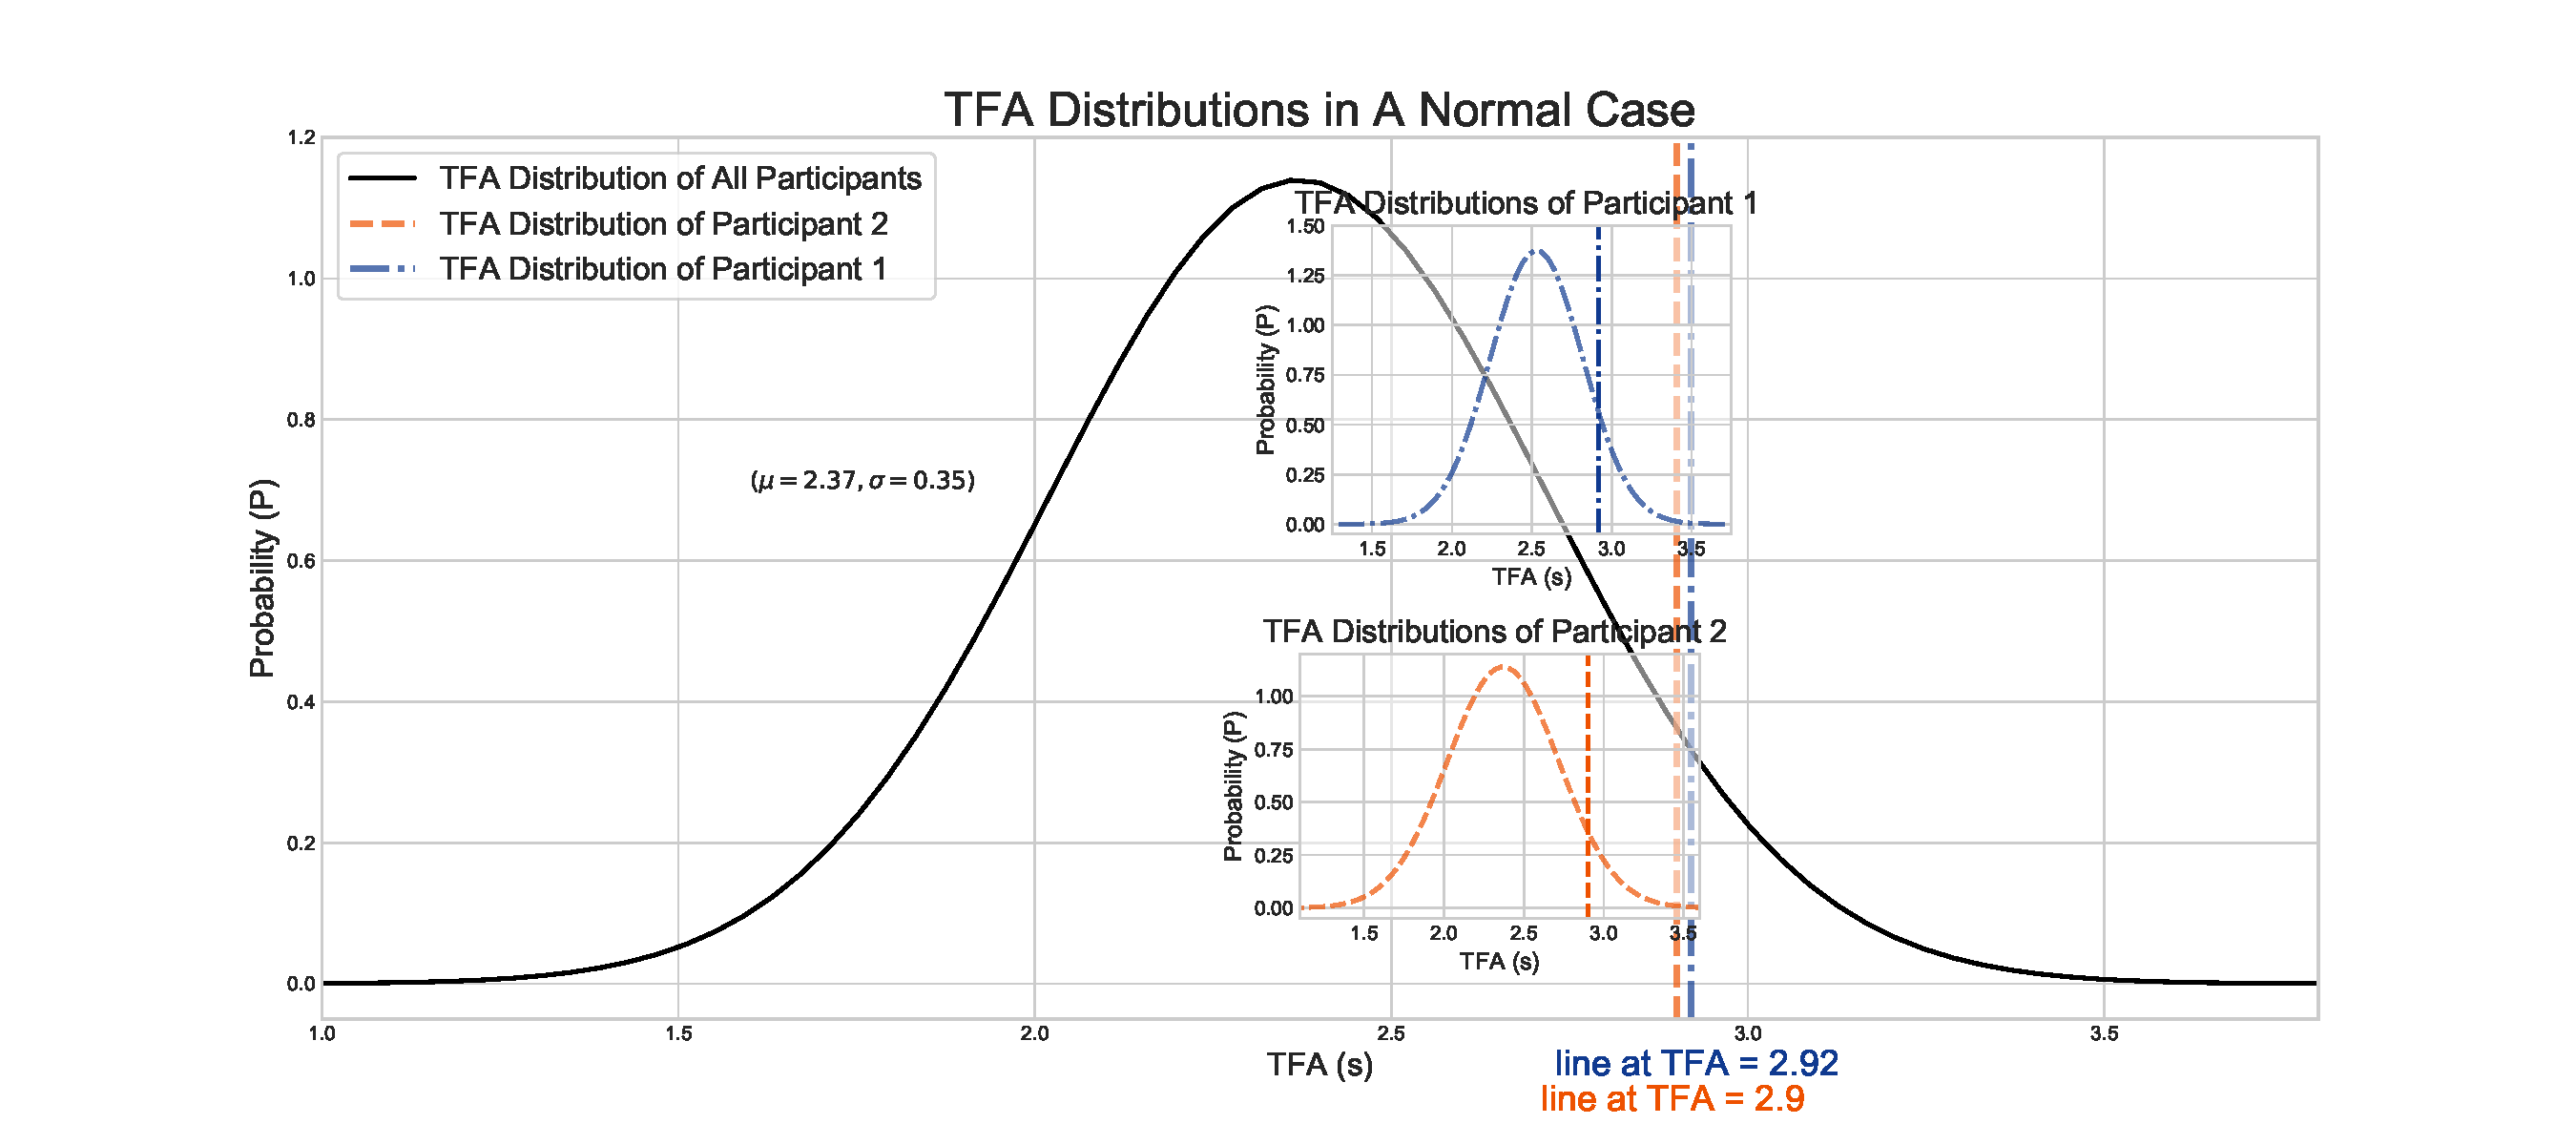
\includegraphics[width=0.9\paperwidth]{/normal015_distributions.pdf}}
\end{center}
\caption{TFA distributions of Participant 1, 2 and average of a normal case where no collision happened.}
\label{fig:TFAs_normal015} 
\end{figure}

The velocities and displacements of both vehicles participated in this case is shown in Fig.~\ref{fig:normal015}, where both vehicles yielded at around  sec to avoid potential collisions from happening. When looking closer at the point of braking of both vehicle, the situation at this moment could be described using the concepts of TFA distributions as shown in Fig.~\ref{fig:TFAs_normal015}. The TFA distribution in black solid line is the average TFA distribution of all people, as illustrated and identified in Chapter \ref{chap:DriverModel}. Two vertical dash lines (all-dash and dash-dot) indicate the TTCs of Car\_0 (the driver is Participant 1) and Car\_1 (the driver is Participant 2) at braking, which are 2.92 and 2.90 respectively (brakes were applied at around 0.7 sec in Fig.~\ref{fig:normal015}). Sub-figures with dashed TFA distributions are the TFA distributions of Participant 1 and 2 (drivers of Car\_0 and Car\_1 respectively). In this case, both drivers brake at the TTC with relatively high likelihood (around 0.4) in the average TFA distribution.

Then, a case where collision happened is shown in Fig.~\ref{fig:accident004} and Fig.~\ref{fig:TFAs_accident004}. Similarly, the velocities and displacements of both vehicles participated in this crashing case is shown in Fig.~\ref{fig:accident004}, however this time, two ehicles collided with each other. 


\begin{figure}[htbp!]
\begin{center}
\makebox[0pt]{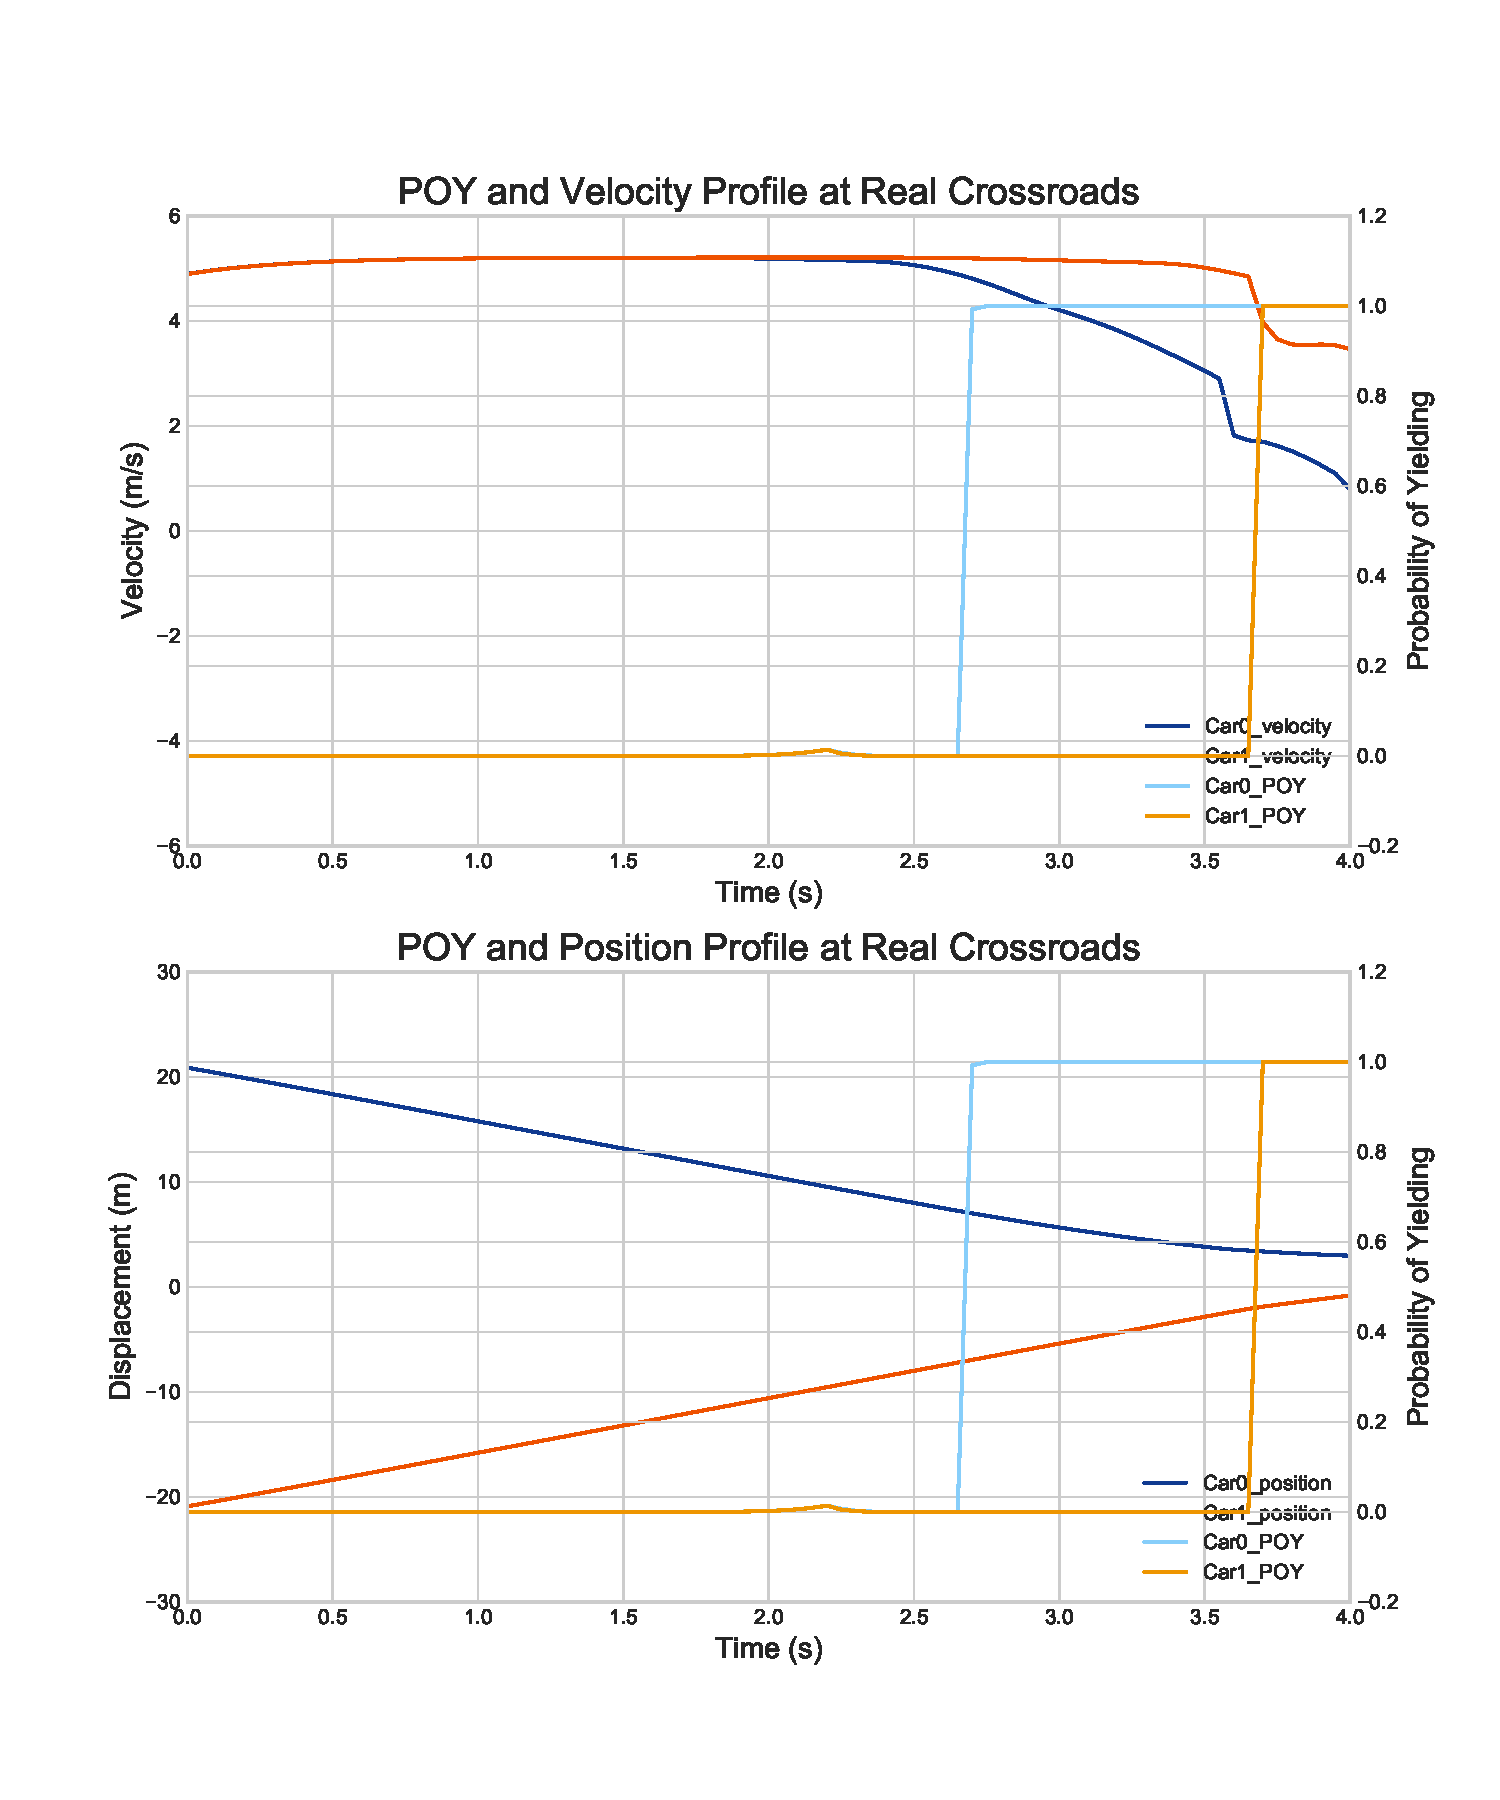
\includegraphics[width=0.65\paperwidth]{/accident_004_aerial.pdf}}
\end{center}
\caption{The velocities and displacements versus POYs of a normal case where a collision did happened.}
\label{fig:accident004} 
\end{figure}

\begin{figure}[htbp!]
\begin{center}
\makebox[0pt]{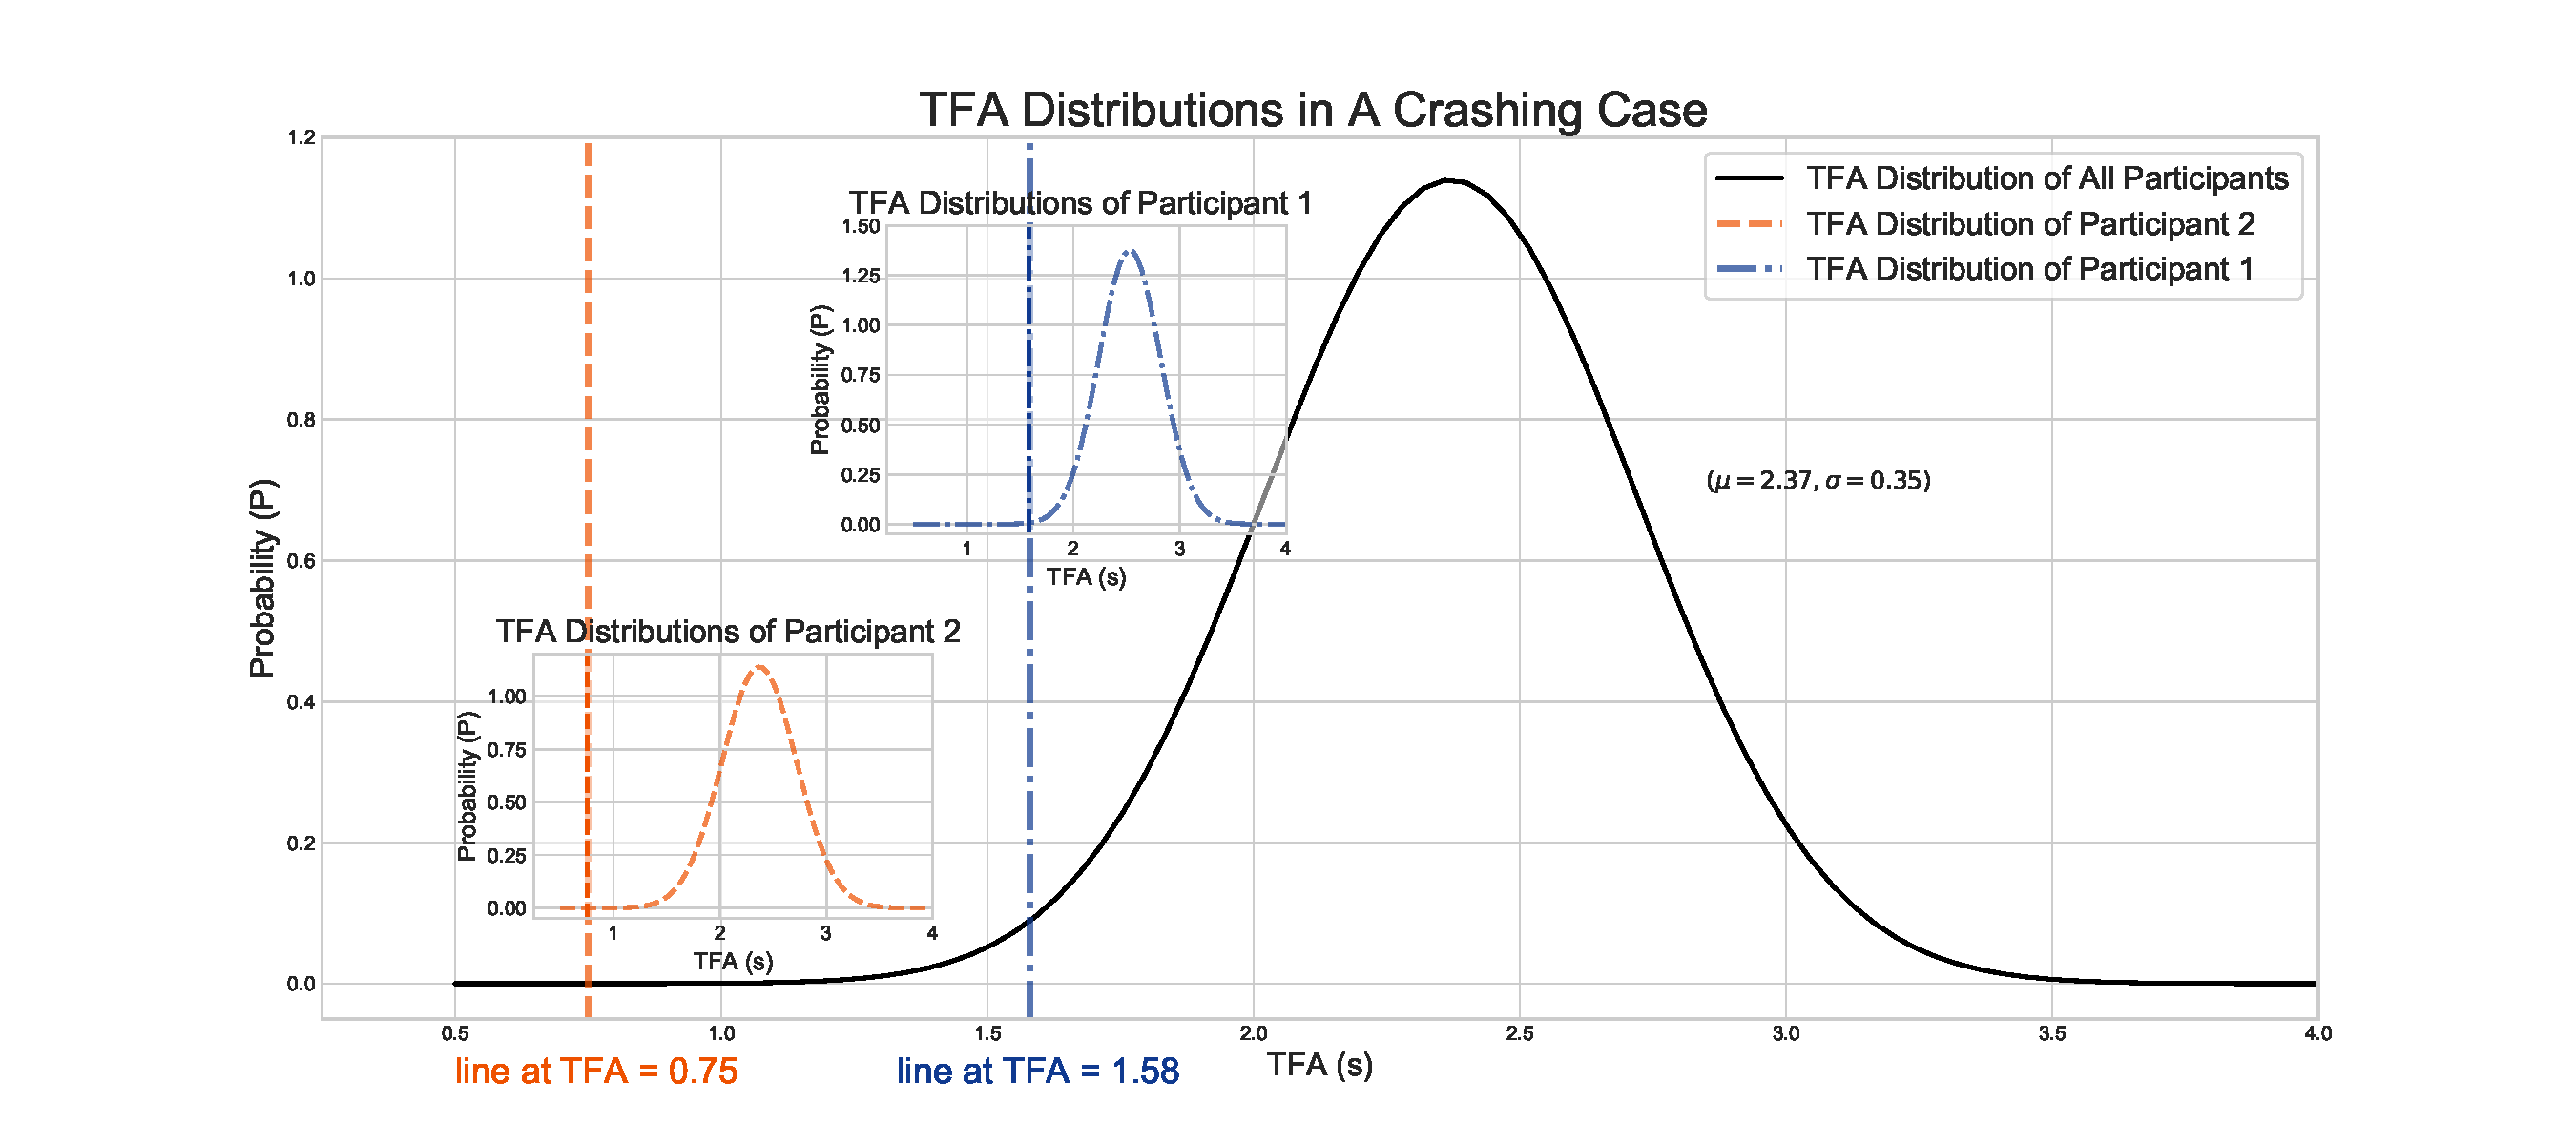
\includegraphics[width=0.9\paperwidth]{/accident004_distributions.pdf}}
\end{center}
\caption{TFA distributions of Participant 1, 2 and average of a normal case where a collision did happened.}
\label{fig:TFAs_accident004} 
\end{figure}


In Fig.~\ref{fig:accident004}, driver of Car\_0 (i.e. Participant 1) believed that the other driver would yield to him, while driver of Car\_1 (i.e. Participant 2) did not even noticed Car\_0 (possibly due to the lack of concentration and obstructions of his view), so they both approached to the intersection with max speed. At around 2.5 sec, Participant 1 finally braked because he realized that the collision was going to happen, and Participant 2 braked at aroundd 3.5 sec, right before the collision. Still, the late braking did not prevent the collision at around 3.6 sec from happening. Then, again, the examination of this scenario using TFA distributions is conducted, as shown in Fig.~\ref{fig:TFAs_accident004}. The figure shows the average TFA distribution in the solid black normal distribution while the TFA distributions of Participant 1 and 2 are shown in dash-dot blue curve and all-dash orange curve respectively. The two dashed lines again indicate the TTCs at the moment of braking for two drivers, which are 0.75 for Participant 2 and 1.50 for Participant 1 respectively. At these TTCs, the likelihoods are both below 0.1, which suggested it is less likely for drivers to brake at these TTC. And the low TTCs also represent aggressive behaviors (brake at shorter distances under the same speed).

Comparing this crashing case (Fig.~\ref{fig:TFAs_accident004}) to the normal case where no collision happened (Fig.~\ref{fig:TFAs_normal015}), we can easily see that in the crashing case, behaviors of drivers tend to be more aggressive (the TFAs of drivers are very low, i.e. they brake at very low TTCs) and they are also less likely to happen (very low likelihood). This finding not only shows that the concept of the proposed model is effective, but also provides a different way to examine the likelihood of accidents happening under some particular behaviors. For example, when drivers at certain crossroads are found to have braking TTCs on the far-left side of the average TFA distribution, it is reasonable to argue that the possibilities of accidents happening in these crossroads are higher due to the more aggressive braking which are also less likely to happen in a normal braking process (the TFA distribution).


%%%%%%%%------------------------------%%%%%%%%%
%%%%%%%%-----------SUBSECTION---------%%%%%%%%%
%%%%%%%%------------------------------%%%%%%%%%
\subsection{TTC differences and POYs}
The differences between the normal and crashing cases can also be distinguished using the TTC differences and the proposed POY. The TTC difference is the difference of the arriving time between two vehicles attempting to cross the intersection at the same time, so smaller the time difference, higher the risk that two vehicles might collide with each other. If either of the vehicles brakes to yielded, the TTC difference will start to expand due to the increasing of the TTC value of the braking vehicle (because the decreasing of the vehicle speed). 

Moreover, the proposed POY can be treated as an index if the weighting term $A_t$ is not applied. Without the weighting term, the POY then rises only when the area under the TFA distribution and right to the current TTC is expending, which indicating that under current TTC, the chances for drivers to brake at that moment is higher. The reason for not using the weighting term $A_t$ is that instead of predicting the behavior of the driver based on his or her current states, only how likely the driver will brake is considered (i.e. whether the driver should brake or not at that TTC).


Combining the TTC difference and the POY without the weighting term, differences between the normal crossing cases and those ending up with collisions at the intersection could be identified. In Fig.~\ref{fig:normal003} and Fig.~\ref{fig:accident004}, the figure at the top is the velocities of the both vehicles shown together with the POY curves without the weighting term, while the figure at the bottom includes the POY curves without the weighting term and the TTC difference indicated in red dashed line. For the cases where pairs of vehicles crossed the intersection without any collision, as shown in Fig.~\ref{fig:normal003}, the POYs without weighting term rose as both vehicles were drove toward the node which means that more and more drivers will brake at this moment to avoid potential collisions. And about 0.5 second before the rise of POYs, the TTC differences rose due to the brake of Car\_0. This rising continued before Car\_1 passed the node. The larger the value of the TTC difference indicating more buffer time and less chance for the collision.


\begin{figure}[htbp!]
\begin{center}
\makebox[0pt]{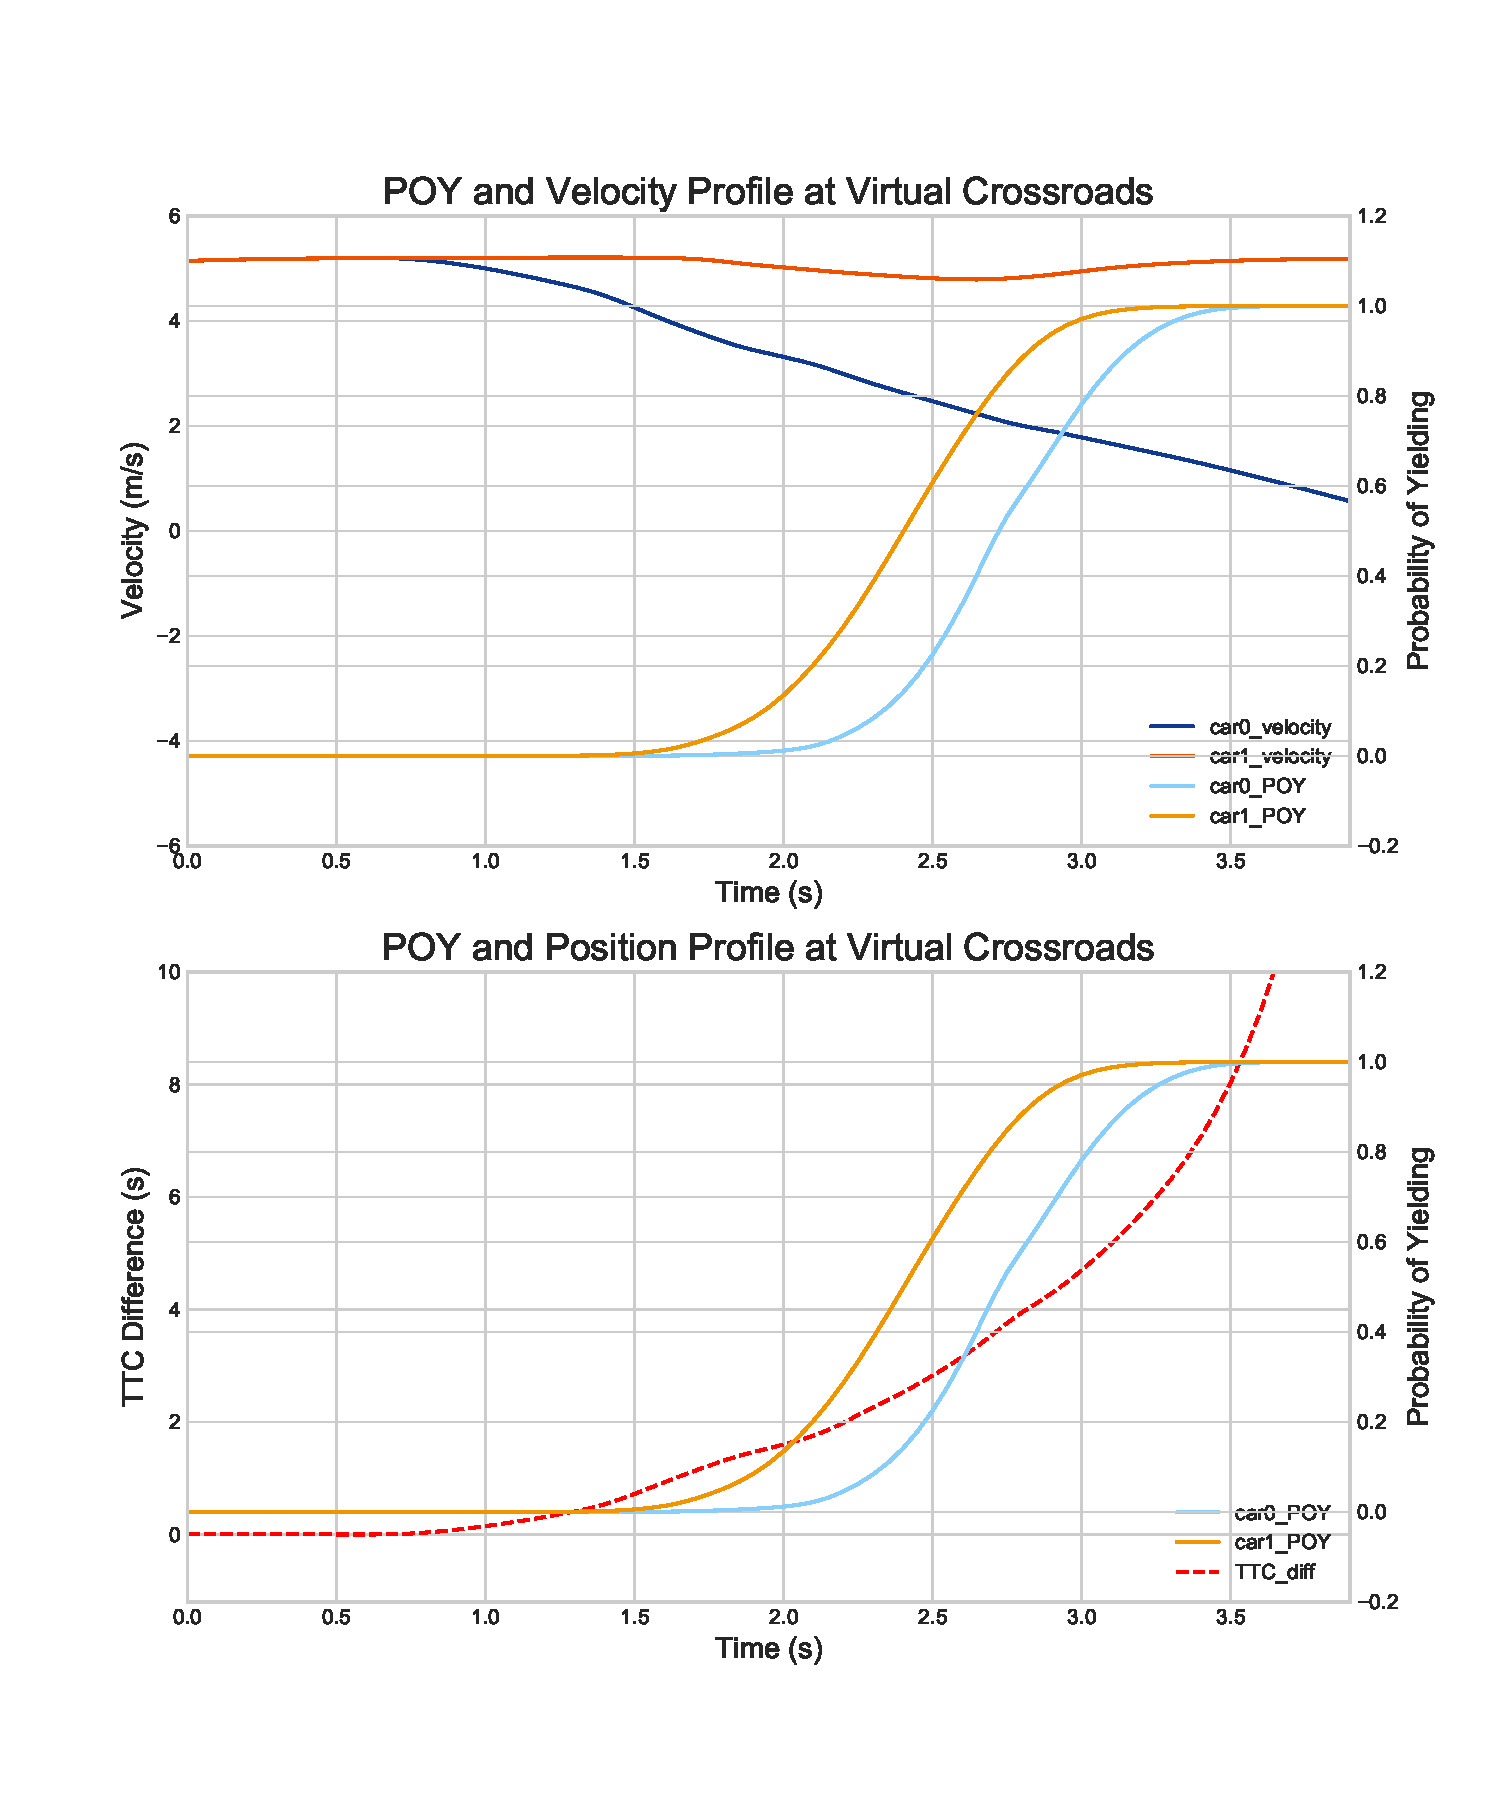
\includegraphics[width=0.65\paperwidth]{normal_003.pdf}}
\end{center}
\caption{Situation where vehicles attempting to cross the intersection passed without any collision. Note that the TTC differences rose before POYs.}
\label{fig:normal003} 
\end{figure}


When it comes to the cases where two vehicles end up colliding with each other, as shown in Fig.~\ref{fig:accident004}, the TTC difference were kept low and did not rise as the POYs were rising. It rose way after the rise of POYs and about 0.8 second before the collision happen owing to the emergency brake was applied. Note the cluttered segments on the velocity lines representing the collision coming right after the emergency brake. In the crashing cases, both vehicles did not notice each other or believed the brake would be applied by the other vehicle, which all end up with crashing at the intersection.

Hence, combining what are observed in both the pass-and-yield cases and the crashing ones, the late-rising TTC difference is highly relevant to the crashing cases. Despite the insufficient data of crashing cases to determine a more accurate TTC difference values and timing that will lead to the crashing, this finding is crucial for identifying the safety index at traffic scenarios. Using this method, it is possible to estimate the risk of accidents according to the driving patterns of the drivers in certain area.


\begin{figure}[htbp!]
\begin{center}
\makebox[0pt]{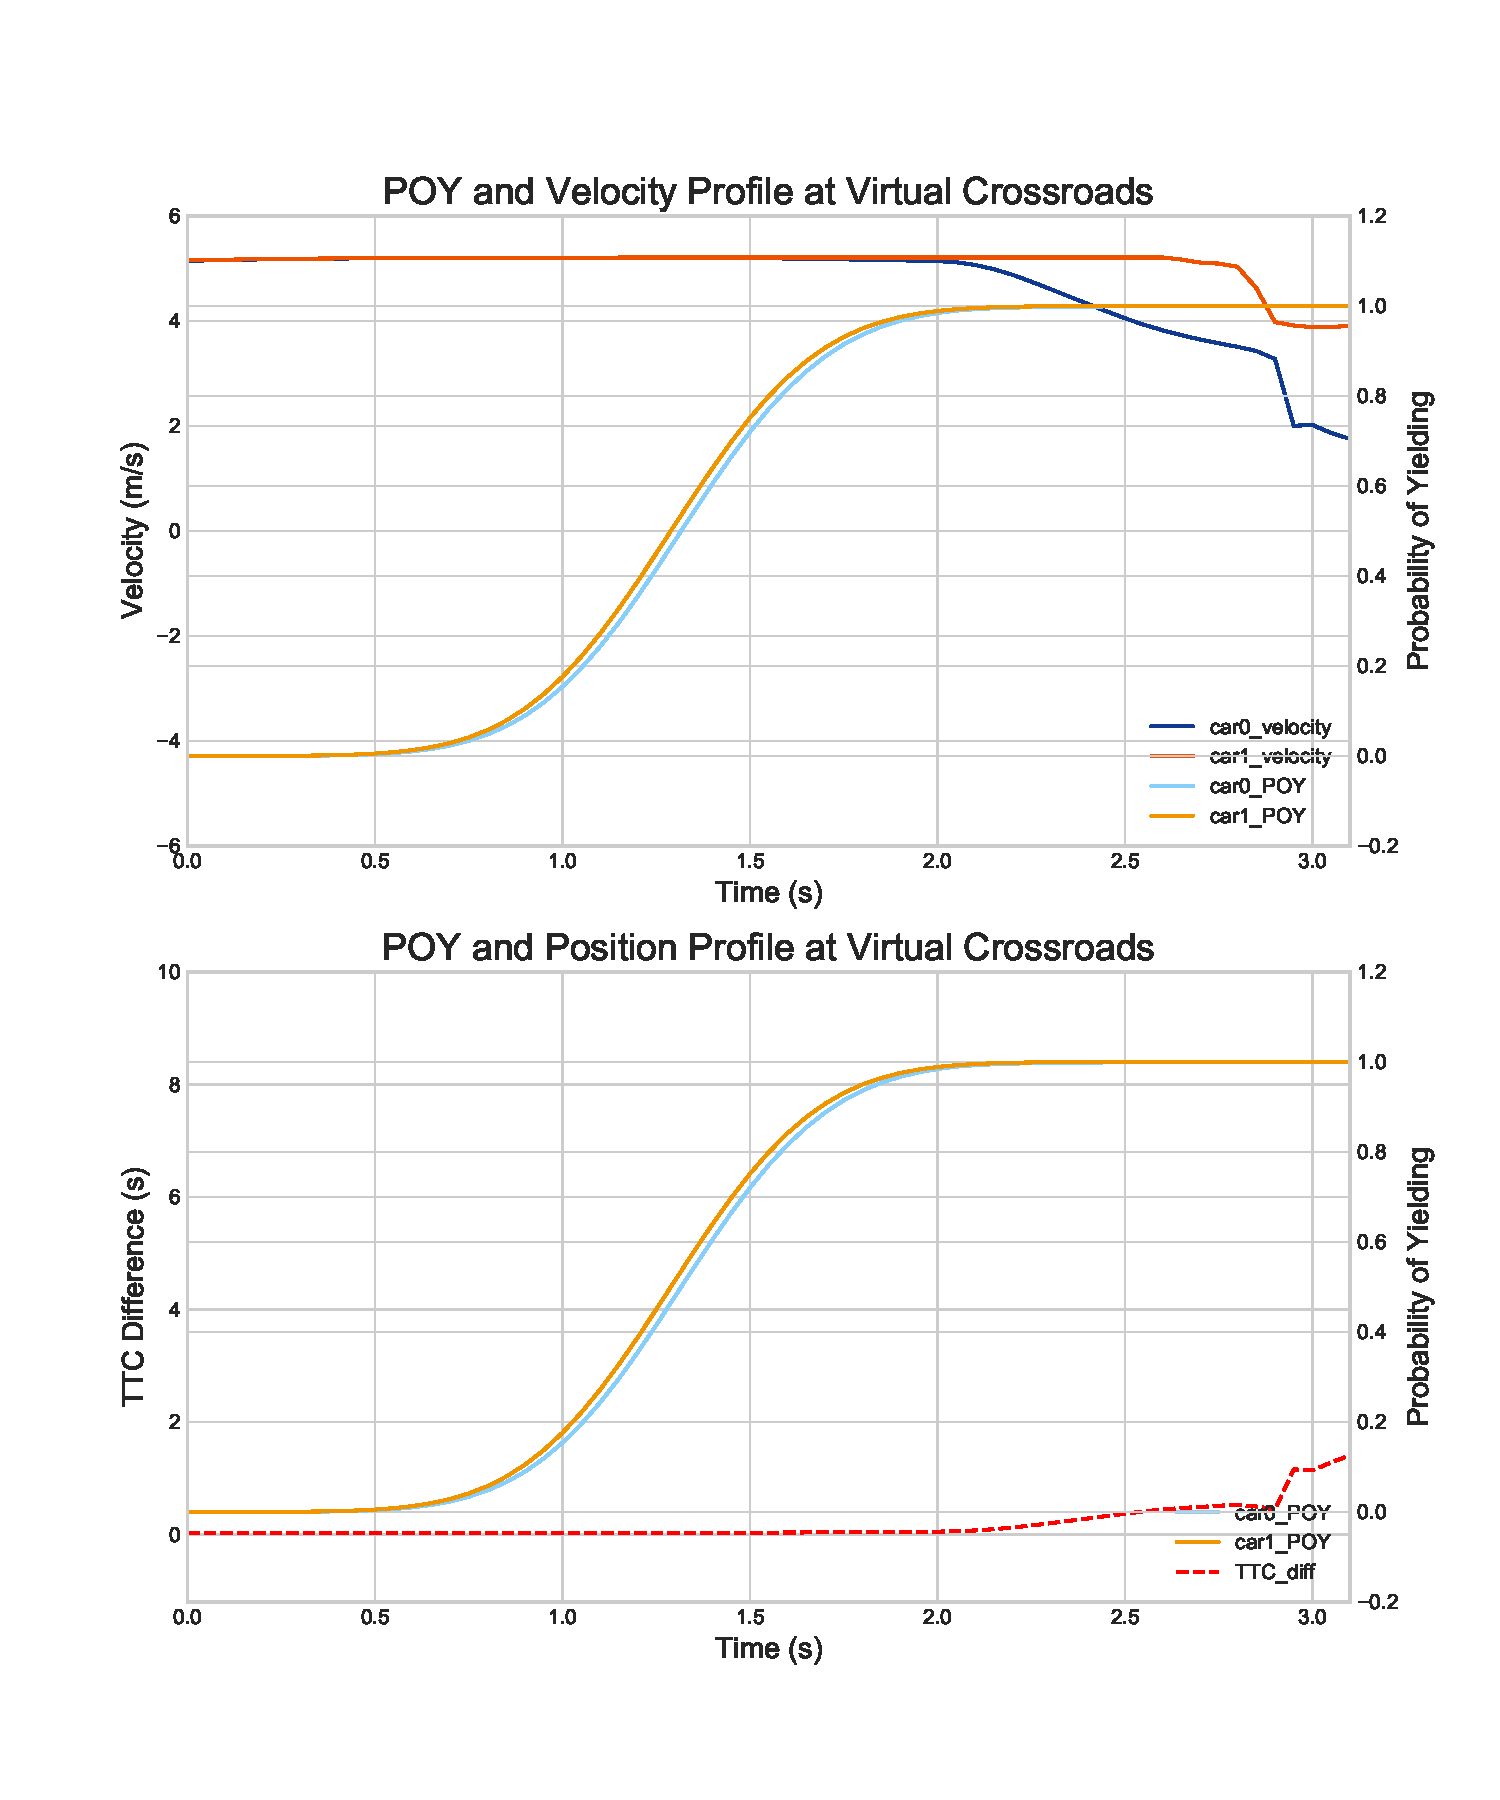
\includegraphics[width=0.65\paperwidth]{accident_004.pdf}}
\end{center}
\caption{Situation where vehicles attempting to cross the intersection collided with each other. Note that the TTC differences rose way after POYs.}
\label{fig:accident004} 
\end{figure}

In this section, possible measures to estimate the possibility of accident happening is proposed. The method uses the TFA distributions to identify the likelihood and the aggressiveness of driver behaviors in certain areas. Then, the TTC differences and the proposed POY are used also to explain the differences between normal and crashing cases. Despite further validations are required, convincing results are provided in both methods and ready to be extended.

%%%%%%%%%%%%%%%%%%%%%%%%%%%%%%%%%%%%%%%%%%%%%%%%%%%%%%%%%%%%%%%%%%%%%%%%
%%%%%%%%%%               SECTION SECTION SECTION               %%%%%%%%%
%%%%%%%%%%%%%%%%%%%%%%%%%%%%%%%%%%%%%%%%%%%%%%%%%%%%%%%%%%%%%%%%%%%%%%%%
\section{POY Estimation at Urban Crossroads}
\label{sec:POY_realCross}

The experiments are conducted to verify whether the proposed POY model can also count for the driver behaviors at the crossroads in real world. In the previous chapter, the importance of characteristic parameter is shown on how the resulting POY curves are affected by different sets of parameters. However, in the complex and stochastic world, to identify the characteristic parameters of all people is impractical and almost impossible, so the average parameter of the participants in the virtual crossroads experiments are adopted in the following experiments, before a more accurate set of parameters that can represent the observed crossroad is identified.

\begin{figure}[htbp!]
\begin{center}
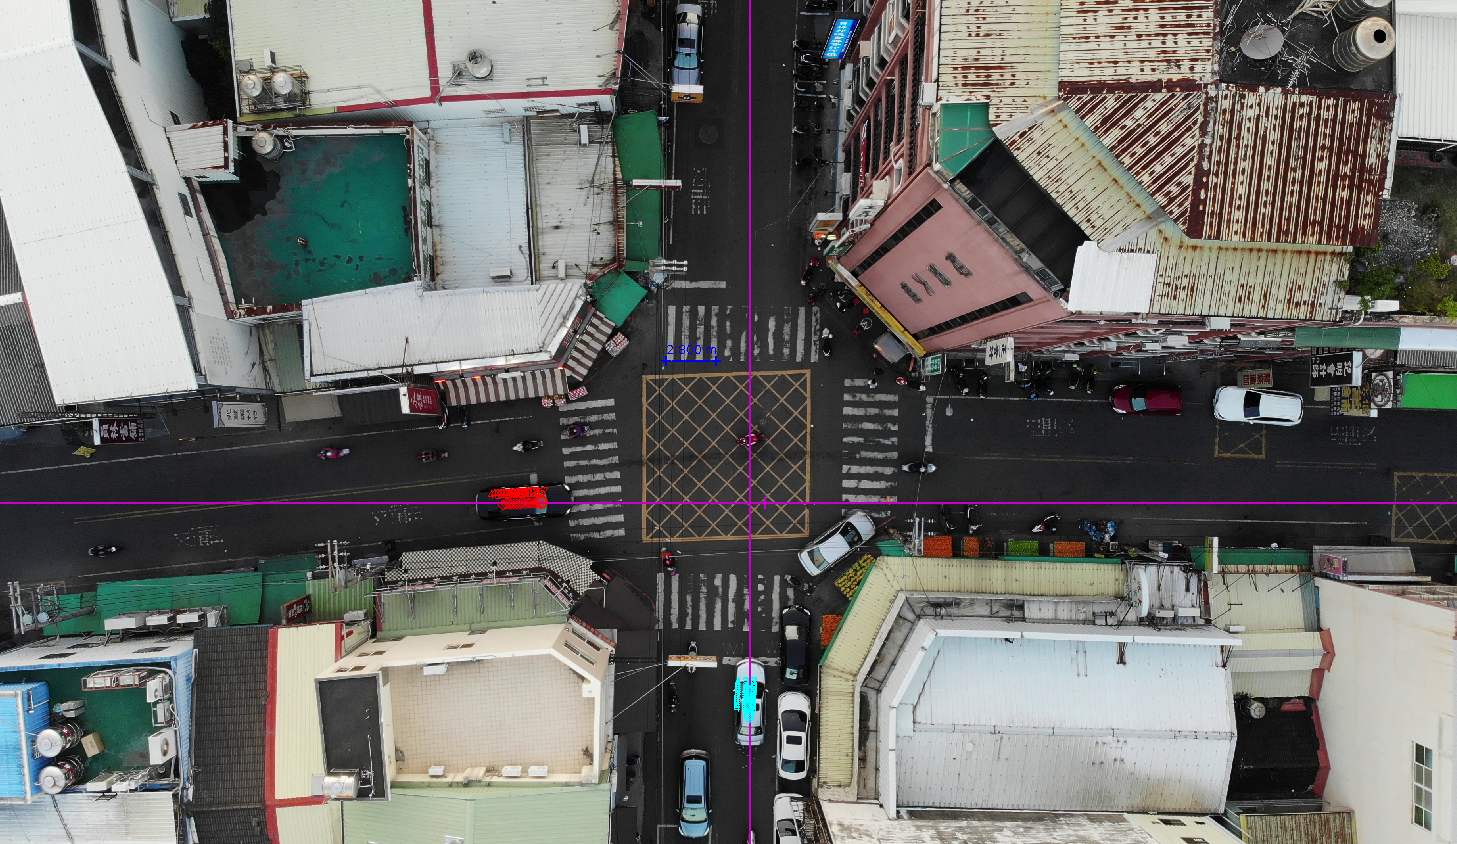
\includegraphics[scale=0.26]{aerial_filming_demo.png}
\end{center}
\caption{Using video analysis tool to track vehicles driven by humans.}
\label{aerial_filming} 
\end{figure}

To collect the related data, the drone for aerial filming is used at the crossroad in urban environment (\textit{Bo’ai Rd.93-85, Yuanlin City, Changhua County 510, Taiwan (23.958606, 120.573283)}). This crossroad is an uncontrolled intersection, where no traffic signal available. To simplify the scenario, cases similar to the assumptions of the proposed model are observed. No turning is allowed and only two participants are involved in the interaction. After the interaction is over, the video analysis tool "tracker" is used to collect and analyze relevant variables ( e.g. velocities and displacements ). The image from the recorded films is shown in Fig.~\ref{aerial_filming}. Note that the angle of the road on the left hand side (about $6.7^\circ$) could be ignored since it only results in approximately 0.1\% difference in velocity. Red and cyan circles indicate the position history of the vehicles at that moment, and the node is set at the intersect of two courses. Interval between every two frames is 0.042 second (24 fps). With the position and the time, the velocity is calculated. To better evaluate the driving behavior, we choose clips with maneuvers of two vehicles that are likely to cause a collision. 

\begin{figure}[htbp!]
\begin{center}
\makebox[0pt]{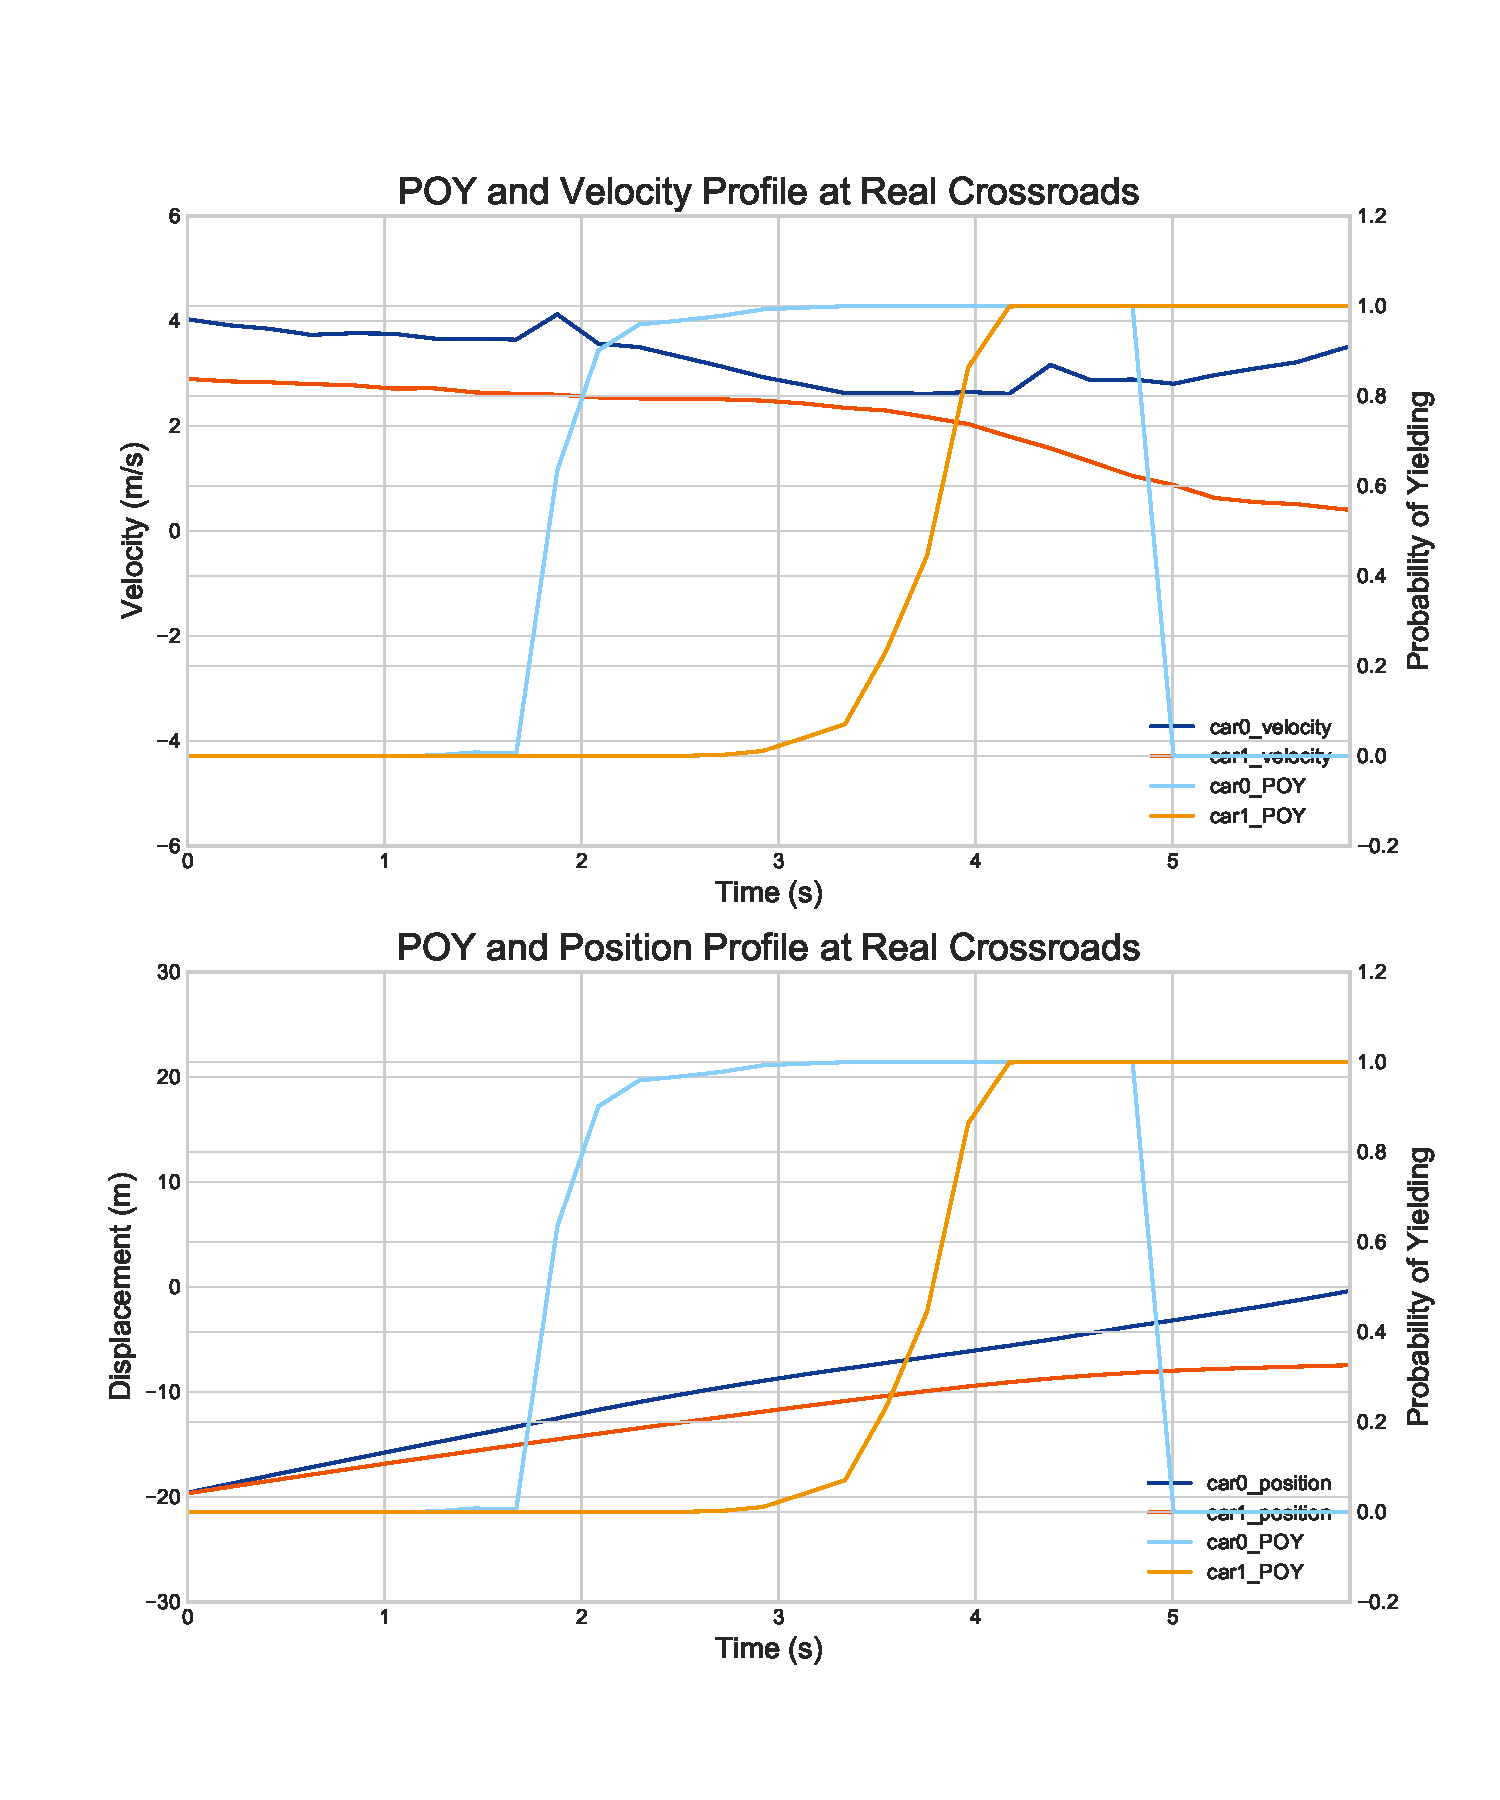
\includegraphics[width=0.65\paperwidth]{realworld_1.pdf}}
\end{center}
\caption{The corresponding POY curve at a crossroad in real world (Case I). car\_0 had the dominance position and passed at the end.}
\label{fig:POY_caseI} 
\end{figure}

Two of the interaction are shown in Fig.~\ref{fig:POY_caseI} and Fig.~\ref{fig:POY_caseII} where the POY curves are similar to those example trials in the virtual crossroads. Owing to the measurement errors for the collected velocity and position profiles, the data shown are smoothen by the means of averaging every 5 collected data. Hence, the derived time step becomes 0.05 sec, which does not exert any influence to the POY estimation.

In the Fig.~\ref{fig:POY_caseI} (case I), the speed of car\_0 was slightly above car\_1 while the displacements to the node were exactly the same at the beginning of the interaction. At around 1.6 sec, the rise of the POY curve of car\_0 was due to the estimated TFA being approached by the lowering TTC. However, this intention was not perceived by the driver of car\_1 because of the subtle difference in their velocities and displacements. After about 1 second later, car\_1 decelerated and decided to yield, causing the rise of the POY curve. The POY of car\_0 then drop to 0 about 1 sec after the car\_1 started to yield. 

\begin{figure}[htbp!]
\begin{center}
\makebox[0pt]{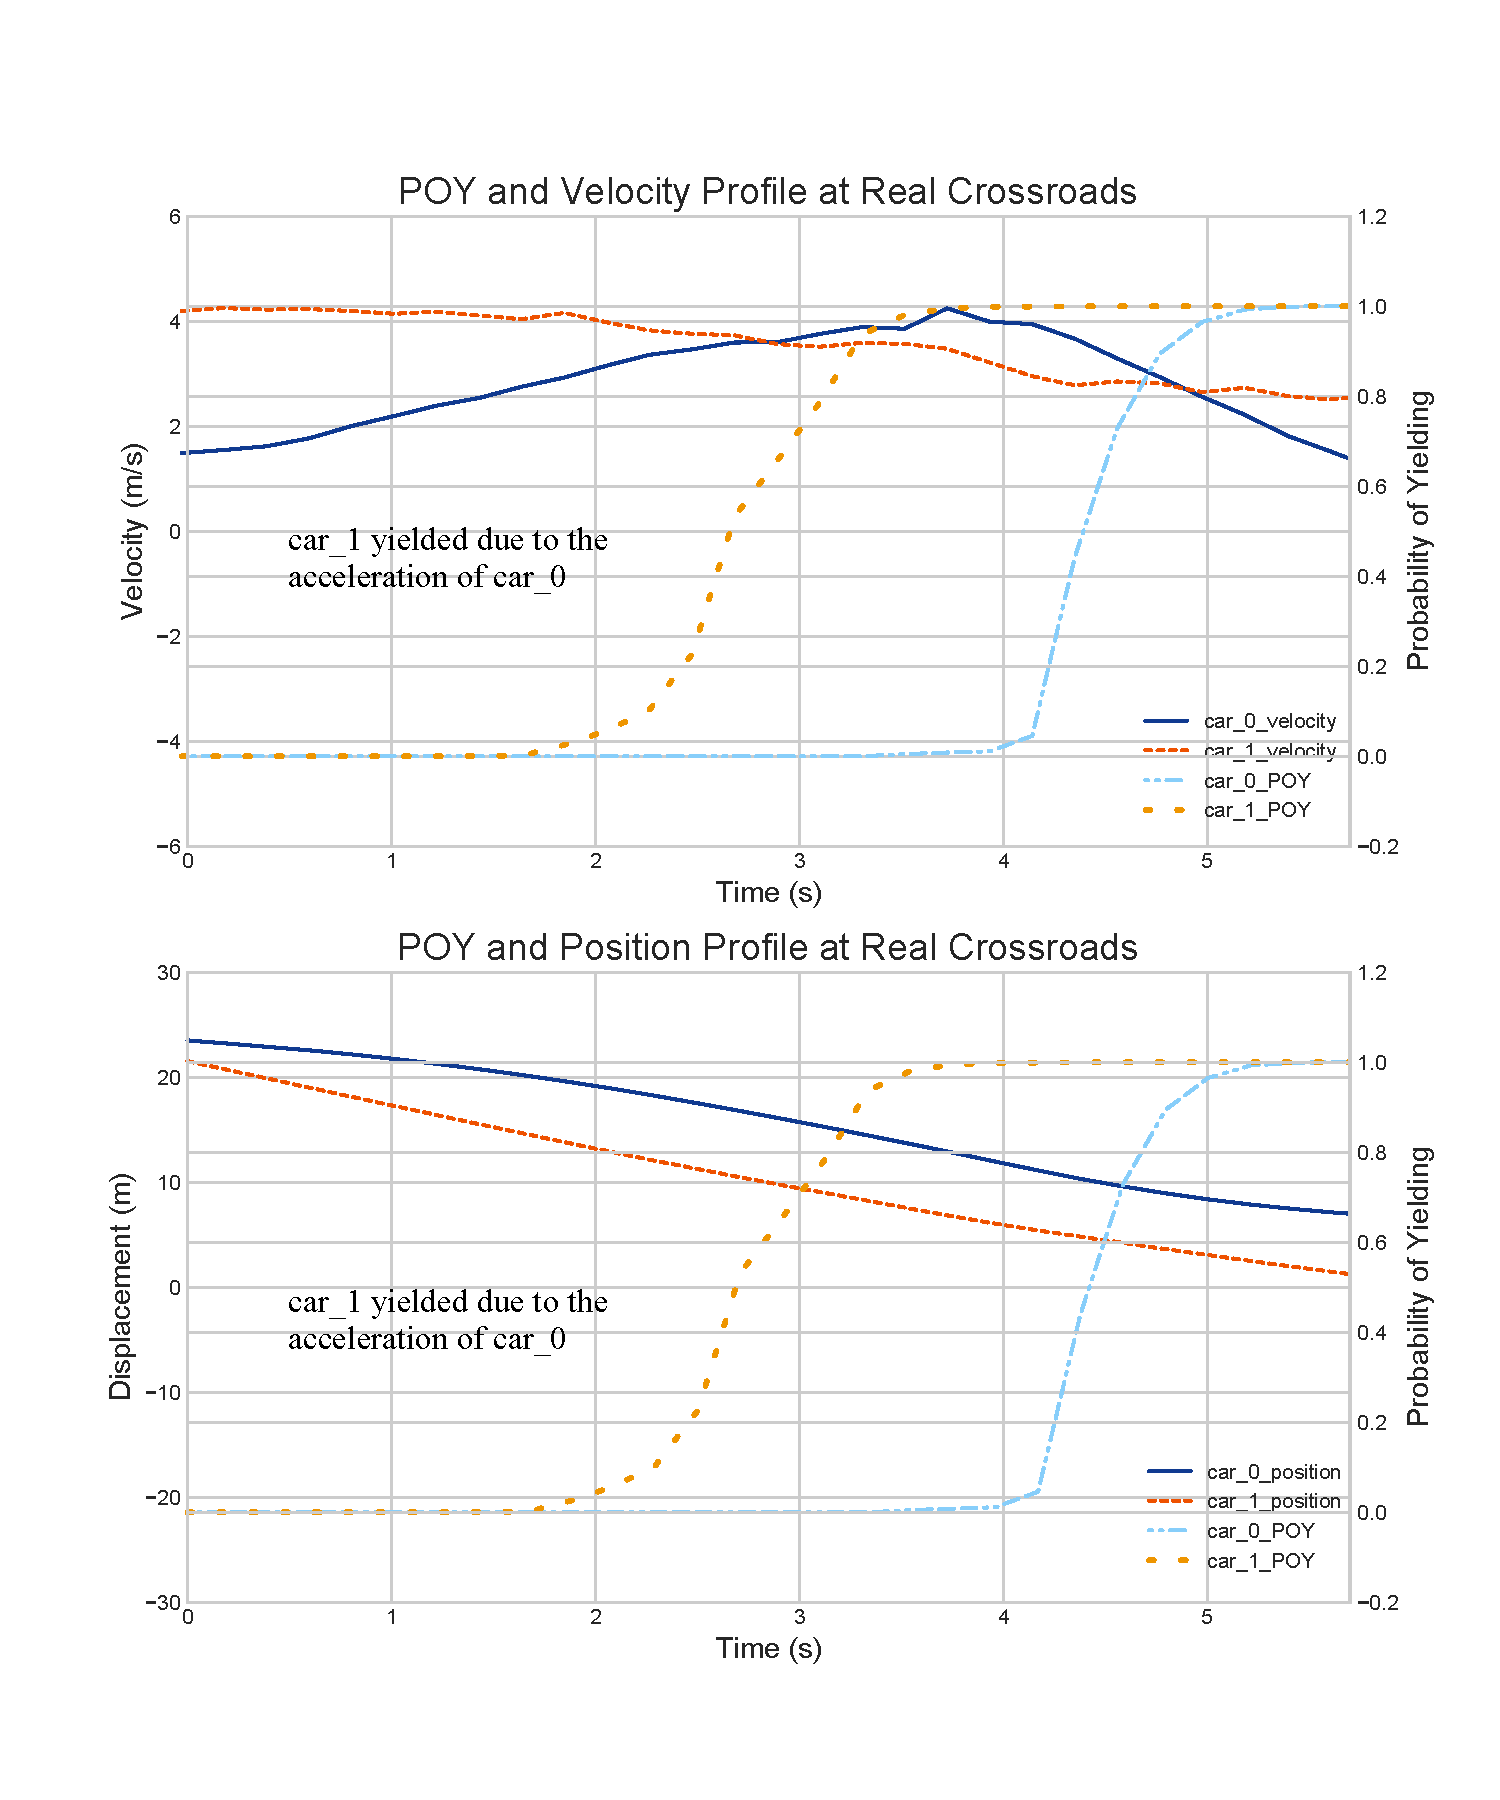
\includegraphics[width=0.65\paperwidth]{realworld_2.pdf}}
\end{center}
\caption{The corresponding POY curve at a crossroad in real world (Case II). car\_1 had the dominance position but yield at the end.}
\label{fig:POY_caseII} 
\end{figure}

There are two possible reasons that car\_1 did not choose to pass at the moment car\_0 begun to yield. First reason is that the intention of the driver of car\_0 was not perceived because of the subtle velocity difference it made. Second reason would be the closer position of car\_0 to the node, which is about 3 meters at the moment car\_1 yielded. So the driver of car\_1 was observing the next decision made by the other driver during 2 to 3.5 sec. But the car\_0 did not make any more obvious move, so car\_1 yielded to avoid possible collision.

In Fig.~\ref{fig:POY_caseII} (case II), car\_1 had faster speed and closer position to the node, but it started decelerating from around 2 sec owing to the acceleration of car\_0. The POY of car\_1 ascended as it decelerated and the TTC had gone closer to the estimated TFA distribution. Till it reached the node, the POY was kept at 1. The possible explanation for this is that car\_1 was much closer to the node (about 6 meters) than car\_0 was, so despite the intention to yield, it did not fully stopped, but was braking very slowly and prepared to yield to the end. 

What can be learned form these two cases are that both cases show similar probabilistic pattern during the observation, which is also comparable to human drivers' prediction. Faster vehicles or vehicles closer to the node (the intersection of the crossroad) are in dominance of crossing over, so despite the intention to yield, they often pass at the end. 

From these two cases,the decisions of human drivers are managed to be turned into probabilistic values and the results are similar to what was done in Chapter~\ref{chap:DriverModel}. However, what the virtual environment can improve to approximate the real one more accurately is that the acceleration values should be set lower or some penalty measures should be taken to keep the participants from driving too recklessly.

\newpage

%%%%%%%%%%%%%%%%%%%%%%%%%%%%%%%%%%%%%%%%%%%%%%%%%%%%%%%%%%%%%%%%%%%%%%%%
%%%%%%%%%%               SECTION SECTION SECTION               %%%%%%%%%
%%%%%%%%%%%%%%%%%%%%%%%%%%%%%%%%%%%%%%%%%%%%%%%%%%%%%%%%%%%%%%%%%%%%%%%%
\section{Procedures for Autonomous Vehicle}
\label{sec:AV_procedure}

Situations are that both driver at the crossroad both yielded at the beginning of the interaction. As we can see in Fig.~\ref{fig:bothyield}, this kind of situations are confusing to human drivers and also autonomous vehicles. For humans, even in the most difficult situation, the solution to this scenario could be a gesture or flashing in the head light. For autonomous vehicles, however, to identify the situation where the other driver is yielding itself poses a problem already.

\begin{figure}[htbp!]
\begin{center}
\makebox[0pt]{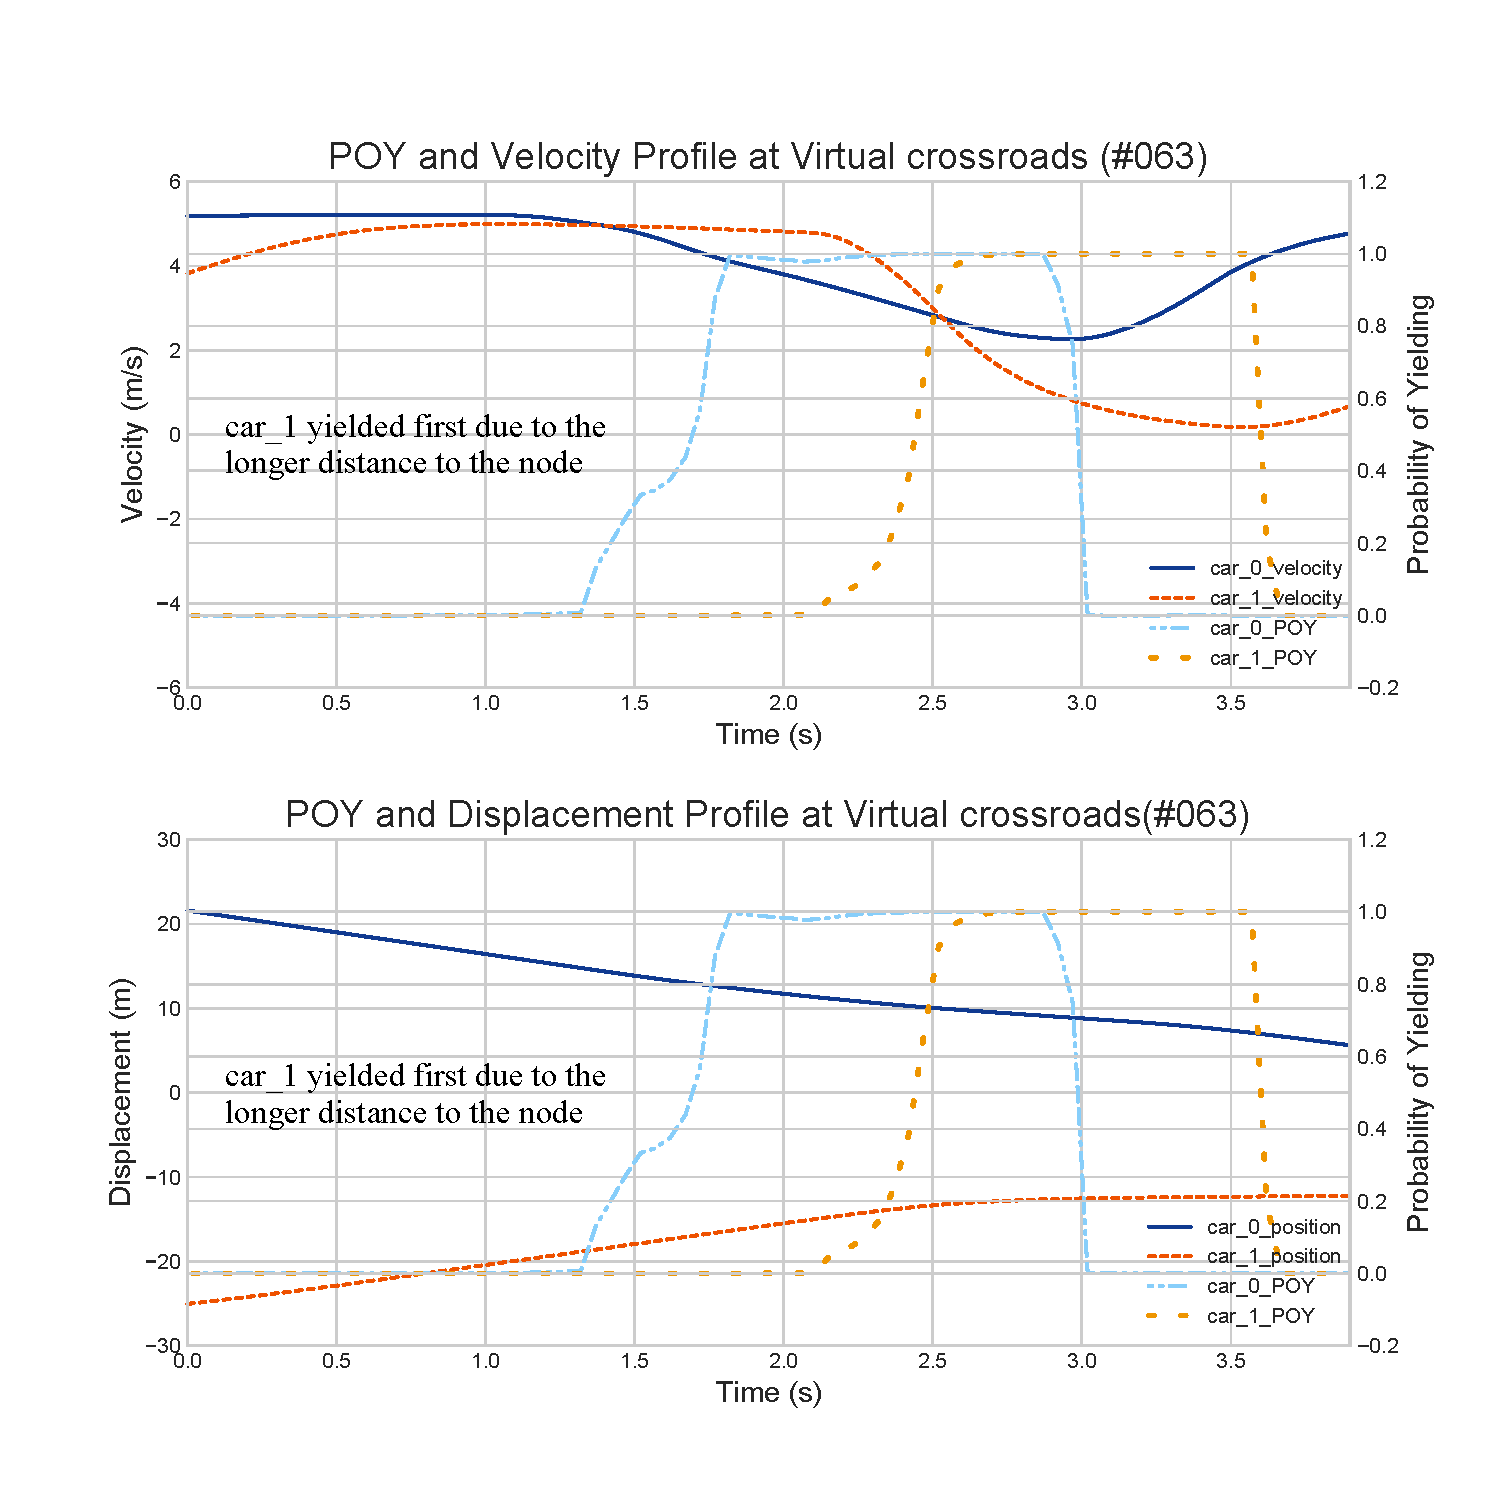
\includegraphics[width=0.65\paperwidth]{trial_063_bothyield.pdf}}
\end{center}
\caption{Both drivers yielded at the beginning of the interaction.}
\label{fig:bothyield} 
\end{figure}

The strategy for autonomous vehicles nowadays to handle the interaction with human is yielding all the time, regardless of the real intentions of the other traffic participant. This kind of behaviors, as mentioned in the Chapter~\ref{chap:Intro}, might lead to collisions since it is not what human drivers usually do. This is where the proposed driver behaviors model comes in handy. With the capability of perceiving the intentions of other traffic participants and present it in a probabilistic way, the POY could be used as a safety measure to handle the situations. 


\begin{figure}[htbp!]
\begin{center}
\makebox[0pt]{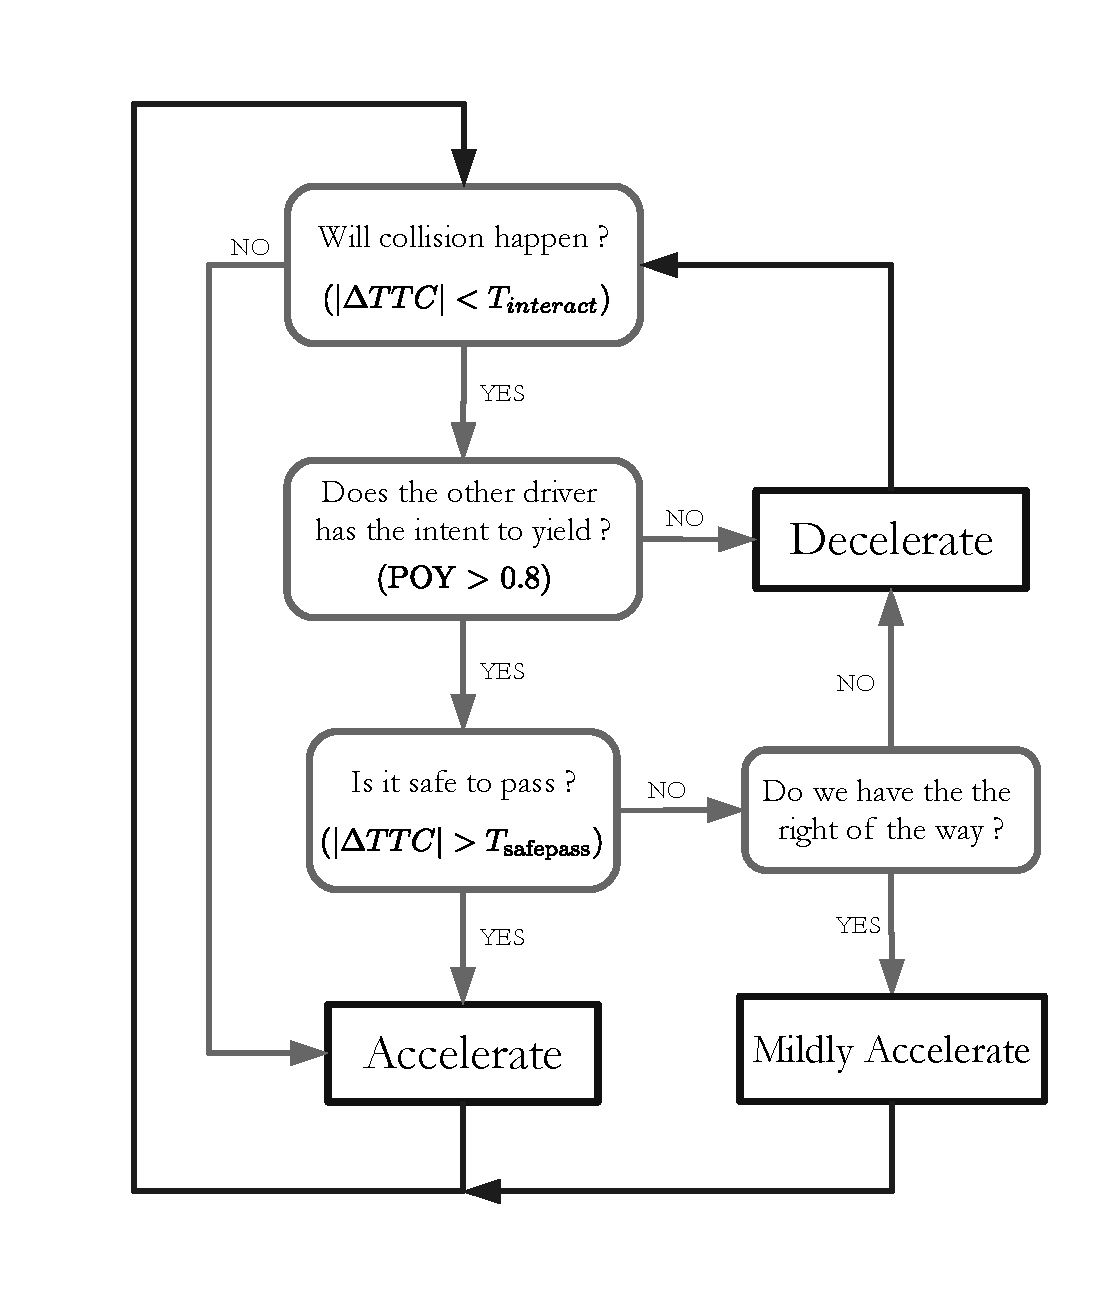
\includegraphics[width=0.53\paperwidth]{/AV_procedure.pdf}}
\end{center}
\caption{Flow chart for autonomous vehicle to deal with the interactions with human drivers.}
\label{fig:flow_chart} 
\end{figure}

When facing complex interactions such as both are yielding, which is similar to the one shown in Fig.~\ref{fig:bothyield}, or when the other vehicle insists on yielding after the autonomous vehicle yield, the process of interaction might take a while, since it is often that both drivers accelerate and decelerate together, leading to a stand off like situation. To allow autonomous vehicle to handle this, a procedure for them to follow is shown in the the flow chart (Fig.~\ref{fig:flow_chart}).

When another traffic participant is detected, the possibility of potential collision happening is first checked. Note that the $\lvert \Delta TTC \rvert$ stands for the absolute value of the difference of TTC between two vehicles. Due to the definition of TTC is the time it takes to arrive at the node, if this difference is smaller than a threshold $T_{interact}$, a collision might happen if no action is taken. Then the POY is checked, where it is defined as yielding if the POY is greater than 0.8 (which is an empirical value). The autonomous vehicle will brake if the other driver intends to pass and will check the $\lvert \Delta TTC \rvert$ again if the other driver intends to yield to make sure the passing is not threatening anyone. At this stage, it is guaranteed for collision-free even if the autonomous vehicle passes without checking the condition $\lvert \Delta TTC \rvert > T_{\text{safepass}}$. However, the smaller the $\lvert \Delta TTC \rvert$, the more dangerous the other driver might feel, hence the threshold $T_{\text{safepass}}$ is defined. For the $\lvert \Delta TTC \rvert$ that might be terrifying to others, the right of the way is then checked, and there will be mild acceleration if the autonomous vehicle has the right of the way. Otherwise the situation will become both yielding, which would spend both parties a considerable amount of time. 

This procedure is applied to the navigation system of one of the simulated vehicle in Gazebo. In Fig.~\ref{fig:POY_HC}, the POY curves during the interaction between human driver and autonomous vehicle (computer driver) are plotted. In this case, both vehicles yielded in the beginning, but as the human driver kept yielding, the computer driver decided to pass. Note that computer driver waited until ($\lvert \Delta TTC \rvert > T_{\text{safepass}}$) before it accelerated.

\begin{figure}[htbp!]
\begin{center}
\makebox[0pt]{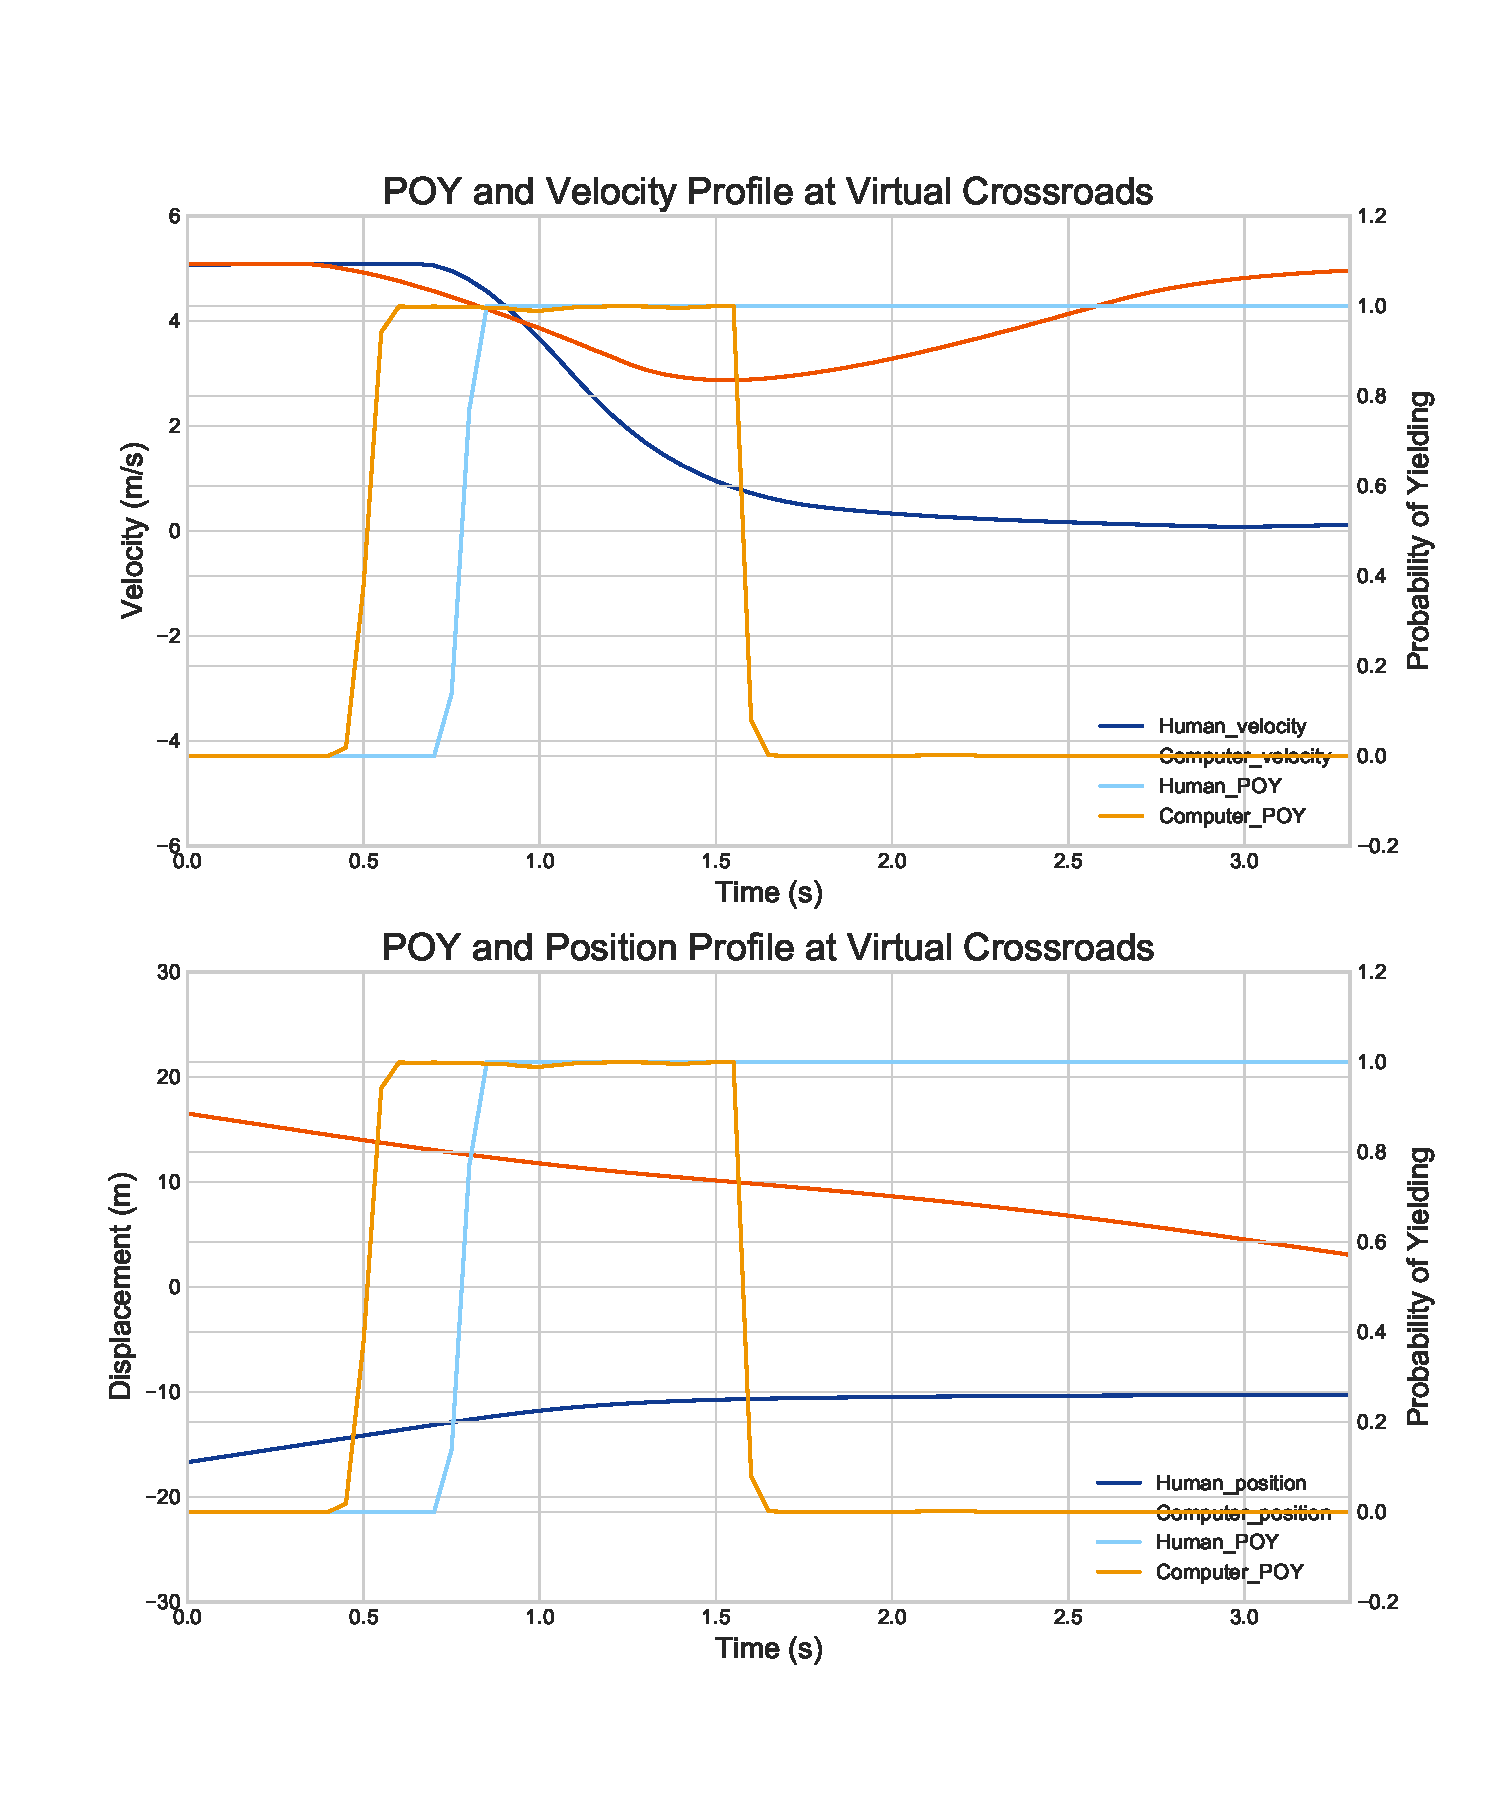
\includegraphics[width=0.65\paperwidth]{HCinteract_2.pdf}}
\end{center}
\caption{The POYs during the interaction between human driver and autonomous vehicle (computer driver) in the simulated environment.}
\label{fig:POY_HC} 
\end{figure}

A few more trials were also conducted to examine the similarity between human drivers and autonomous vehicles following this procedure. Human contestants were asked to drive across the virtual crossroad as in the previous experiments without knowing that the other vehicle was actually an autonomous vehicle with the proposed navigation system. Almost all the contestants did not realize it was the autonomous vehicle they were interacting. Even though the experiments were not assessed thorough enough, it is an initiation to make autonomous vehicles drive more like human. 


\begin{figure}[htbp!]
\begin{center}
\makebox[0pt]{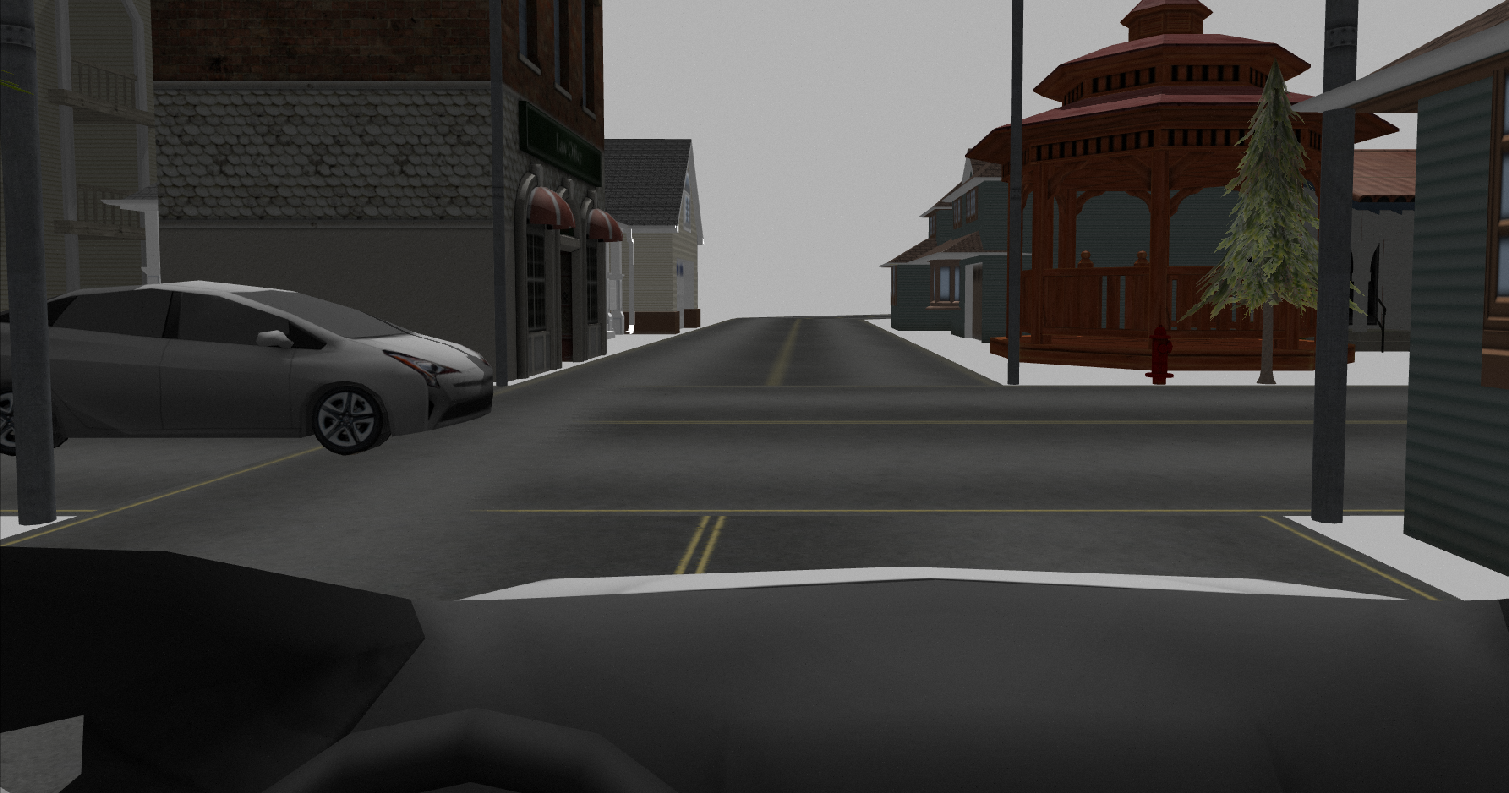
\includegraphics[width=0.6\paperwidth]{AV_interaction.png}}
\end{center}
\caption{The scene of interaction between human driver and autonomous vehicle with navigation algorithm in the simulated environment.}
\label{fig:screenshot_AVinteraction} 
\end{figure}


%%%%%%%%%%%%%%%%%%%%%%%%%%%%%%%%%%%%%%%%%%%%%%%%%%%%%%%%%%%%%%%%%%%%%%%%
%%%%%%%%%%               SECTION SECTION SECTION               %%%%%%%%%
%%%%%%%%%%%%%%%%%%%%%%%%%%%%%%%%%%%%%%%%%%%%%%%%%%%%%%%%%%%%%%%%%%%%%%%%
%\section{Driver Parameters Identification at Urban Crossroads}
%\label{sec:ParamID_realCross}


In this chapter, the possible applications for the proposed model are explored. First, the crashing cases were identified to be highly related to certain aggressive driver behaviors. Then, proposed POY was used to evaluate the intentions of drivers at crossroads in real world. The result are similar to those observed and verified in the simulated environment. Then, a procedure was defined to allow autonomous vehicle to have a more efficient and smooth interaction process when facing difficult situations. These applications will be further extended to finally apply on a real autonomous devices. 